\setLayout{vertical}
\subsection{Descrizione della nuova interfaccia}
\begin{frame}
    \frametitle{Descrizione della nuova interfaccia}
    L'interfaccia risultante dalla nostra riprogettazione si articola in quattro schermate: 
    \begin{itemize}
        \item \hyperlink{panoramica}{Panoramica} 
        \item \hyperlink{confronto-regioni}{Confronto fra regioni}
        \item \hyperlink{analisi-periodi}{Analisi di periodi}
        \item \hyperlink{distribuzione}{Distribuzione su dati anagrafici}
    \end{itemize}  

\end{frame}

\begin{frame}
    \frametitle{Panoramica}
    \label{panoramica}
    \begin{figure}
        \centering
        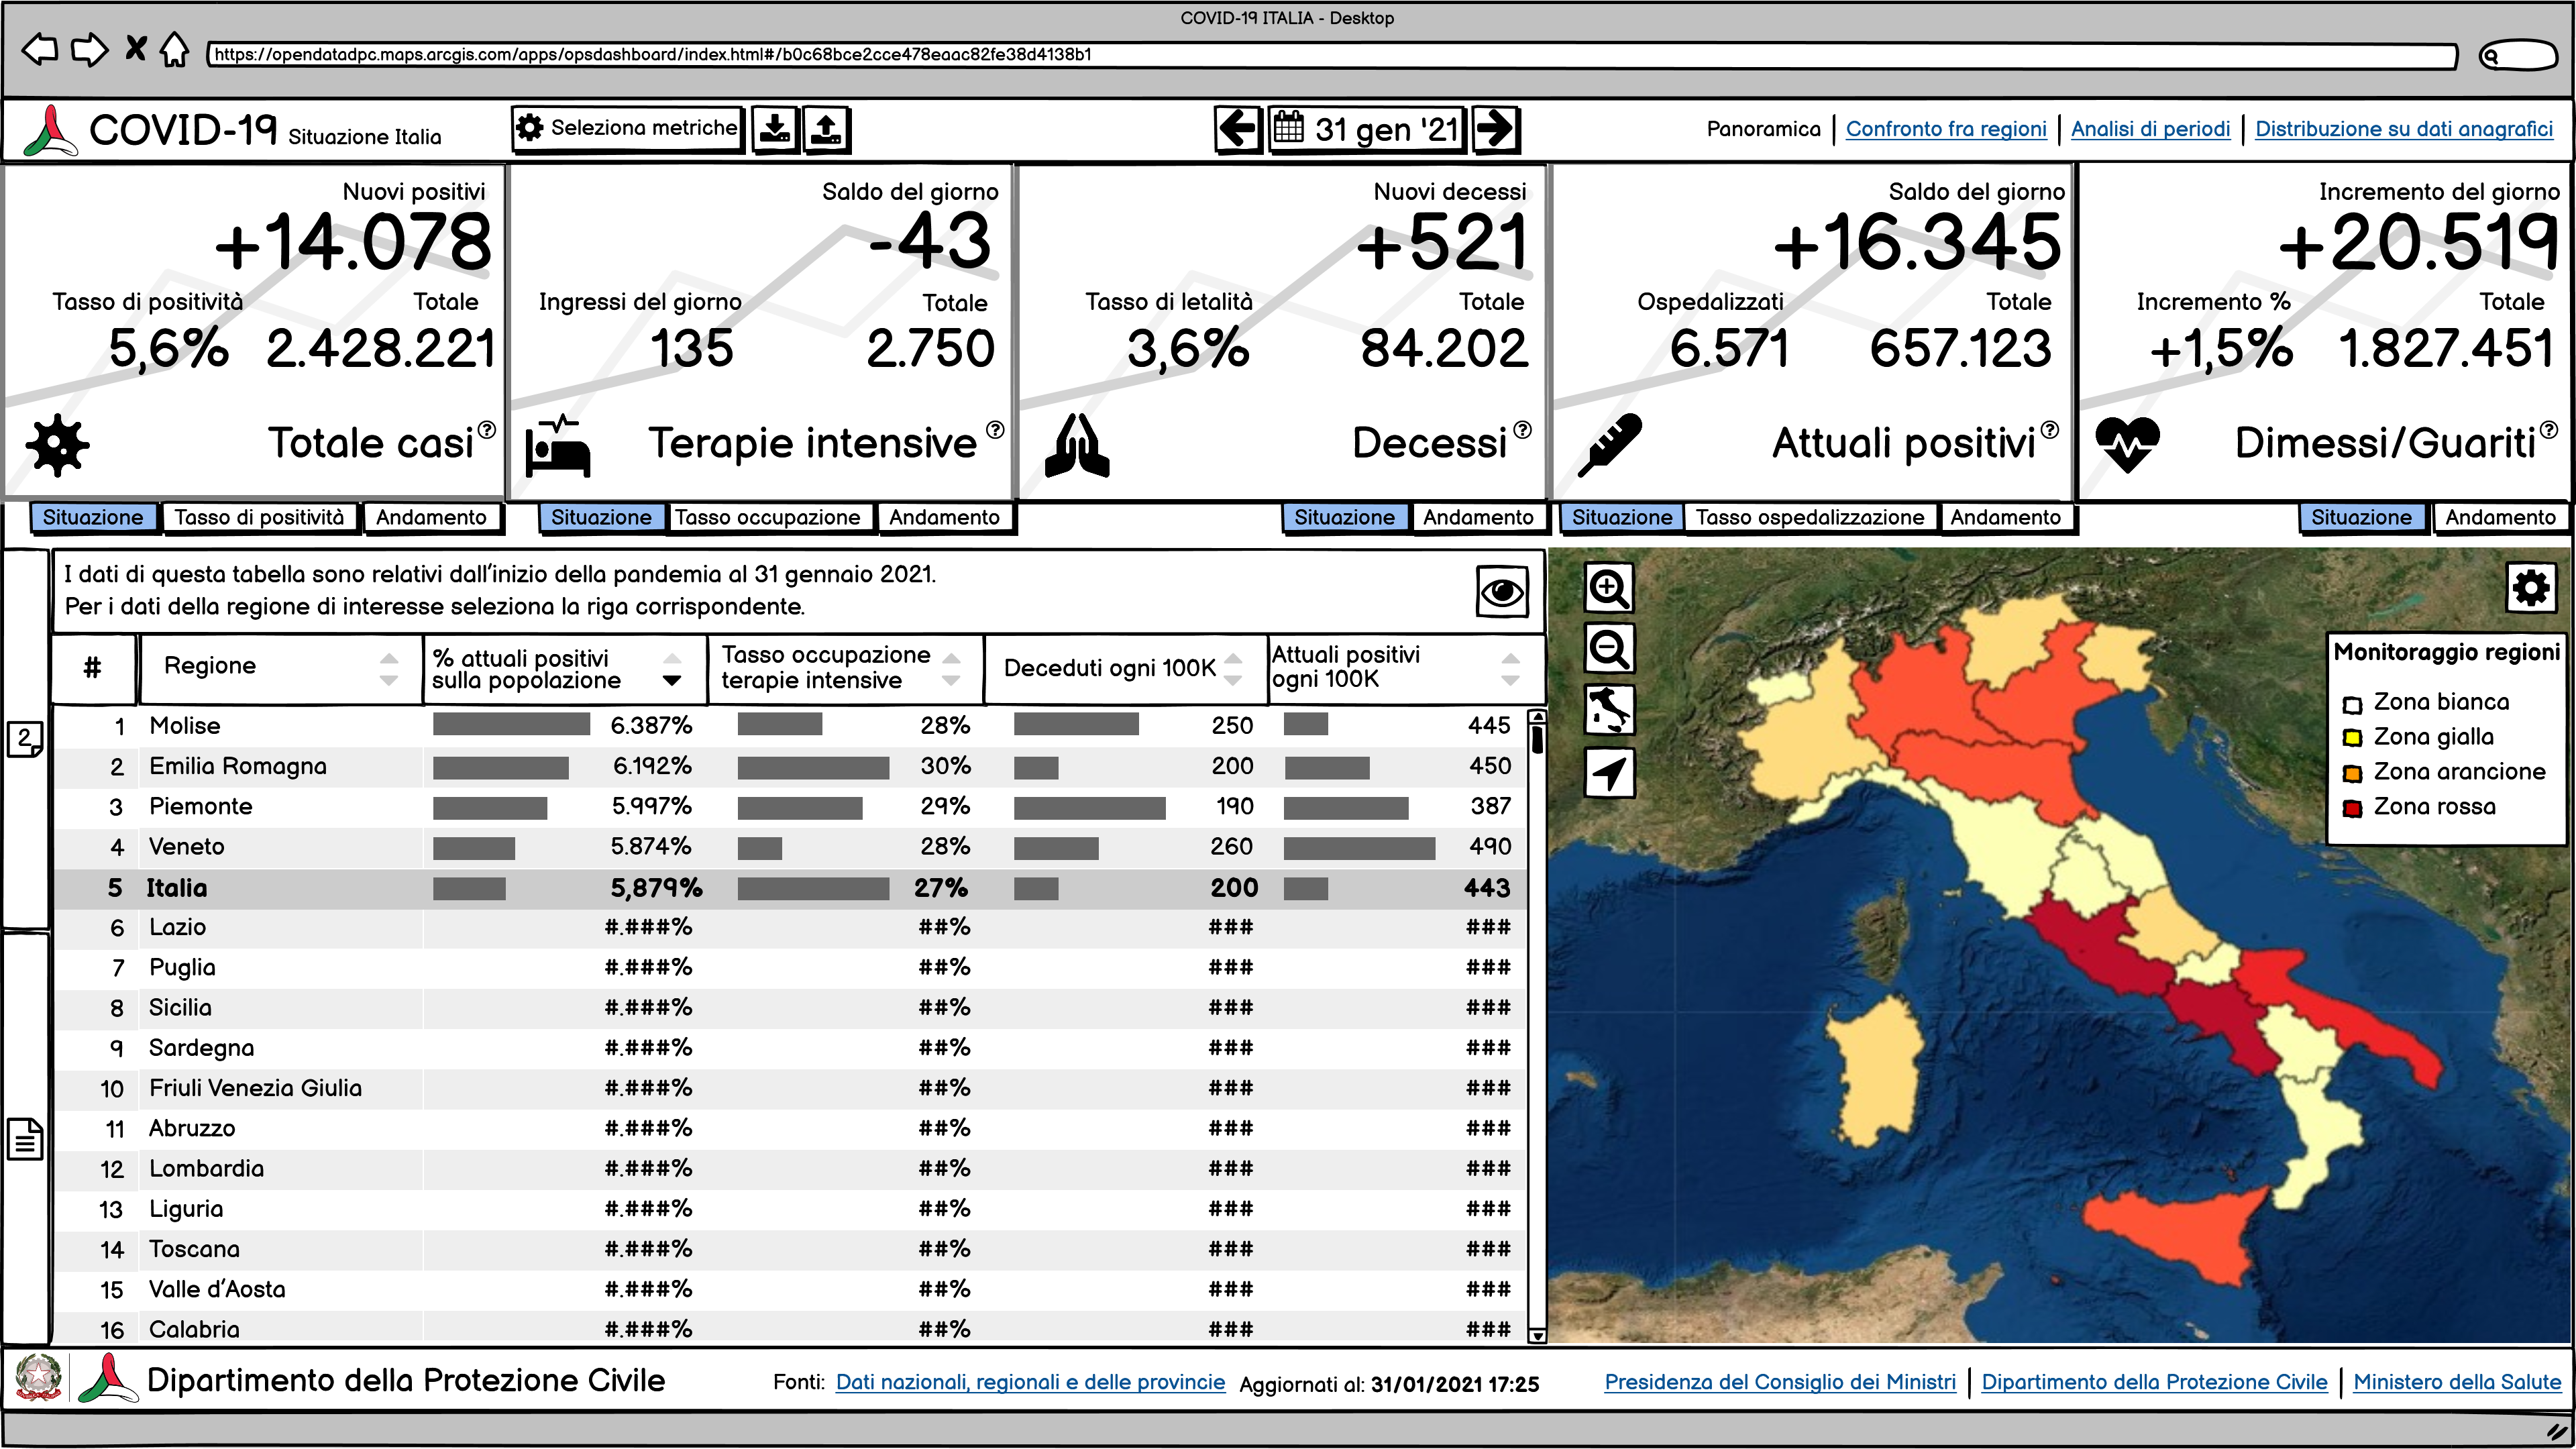
\includegraphics[width=.8\textwidth]{screen-interfaccia/1 - Panoramica.png}
        \caption{Schermata "Panoramica" dell'interfaccia riprogettata.}
    \end{figure}
    
\end{frame}

\begin{frame}
    \frametitle{Panoramica - Box numerici}
    La parte superiore visualizza dei box, ciascuno dei quali presenta delle schede selezionabili: in linea generale, in essi il giornalista potrà avere un colpo d'occhio sui totali delle metriche fondamentali e sulle loro variazioni rispetto al giorno precedente a quello specificato, nonché indicatori di livello o curve del loro andamento nel periodo temporale indicato mediante gli slider.
    \begin{figure}
        \centering
        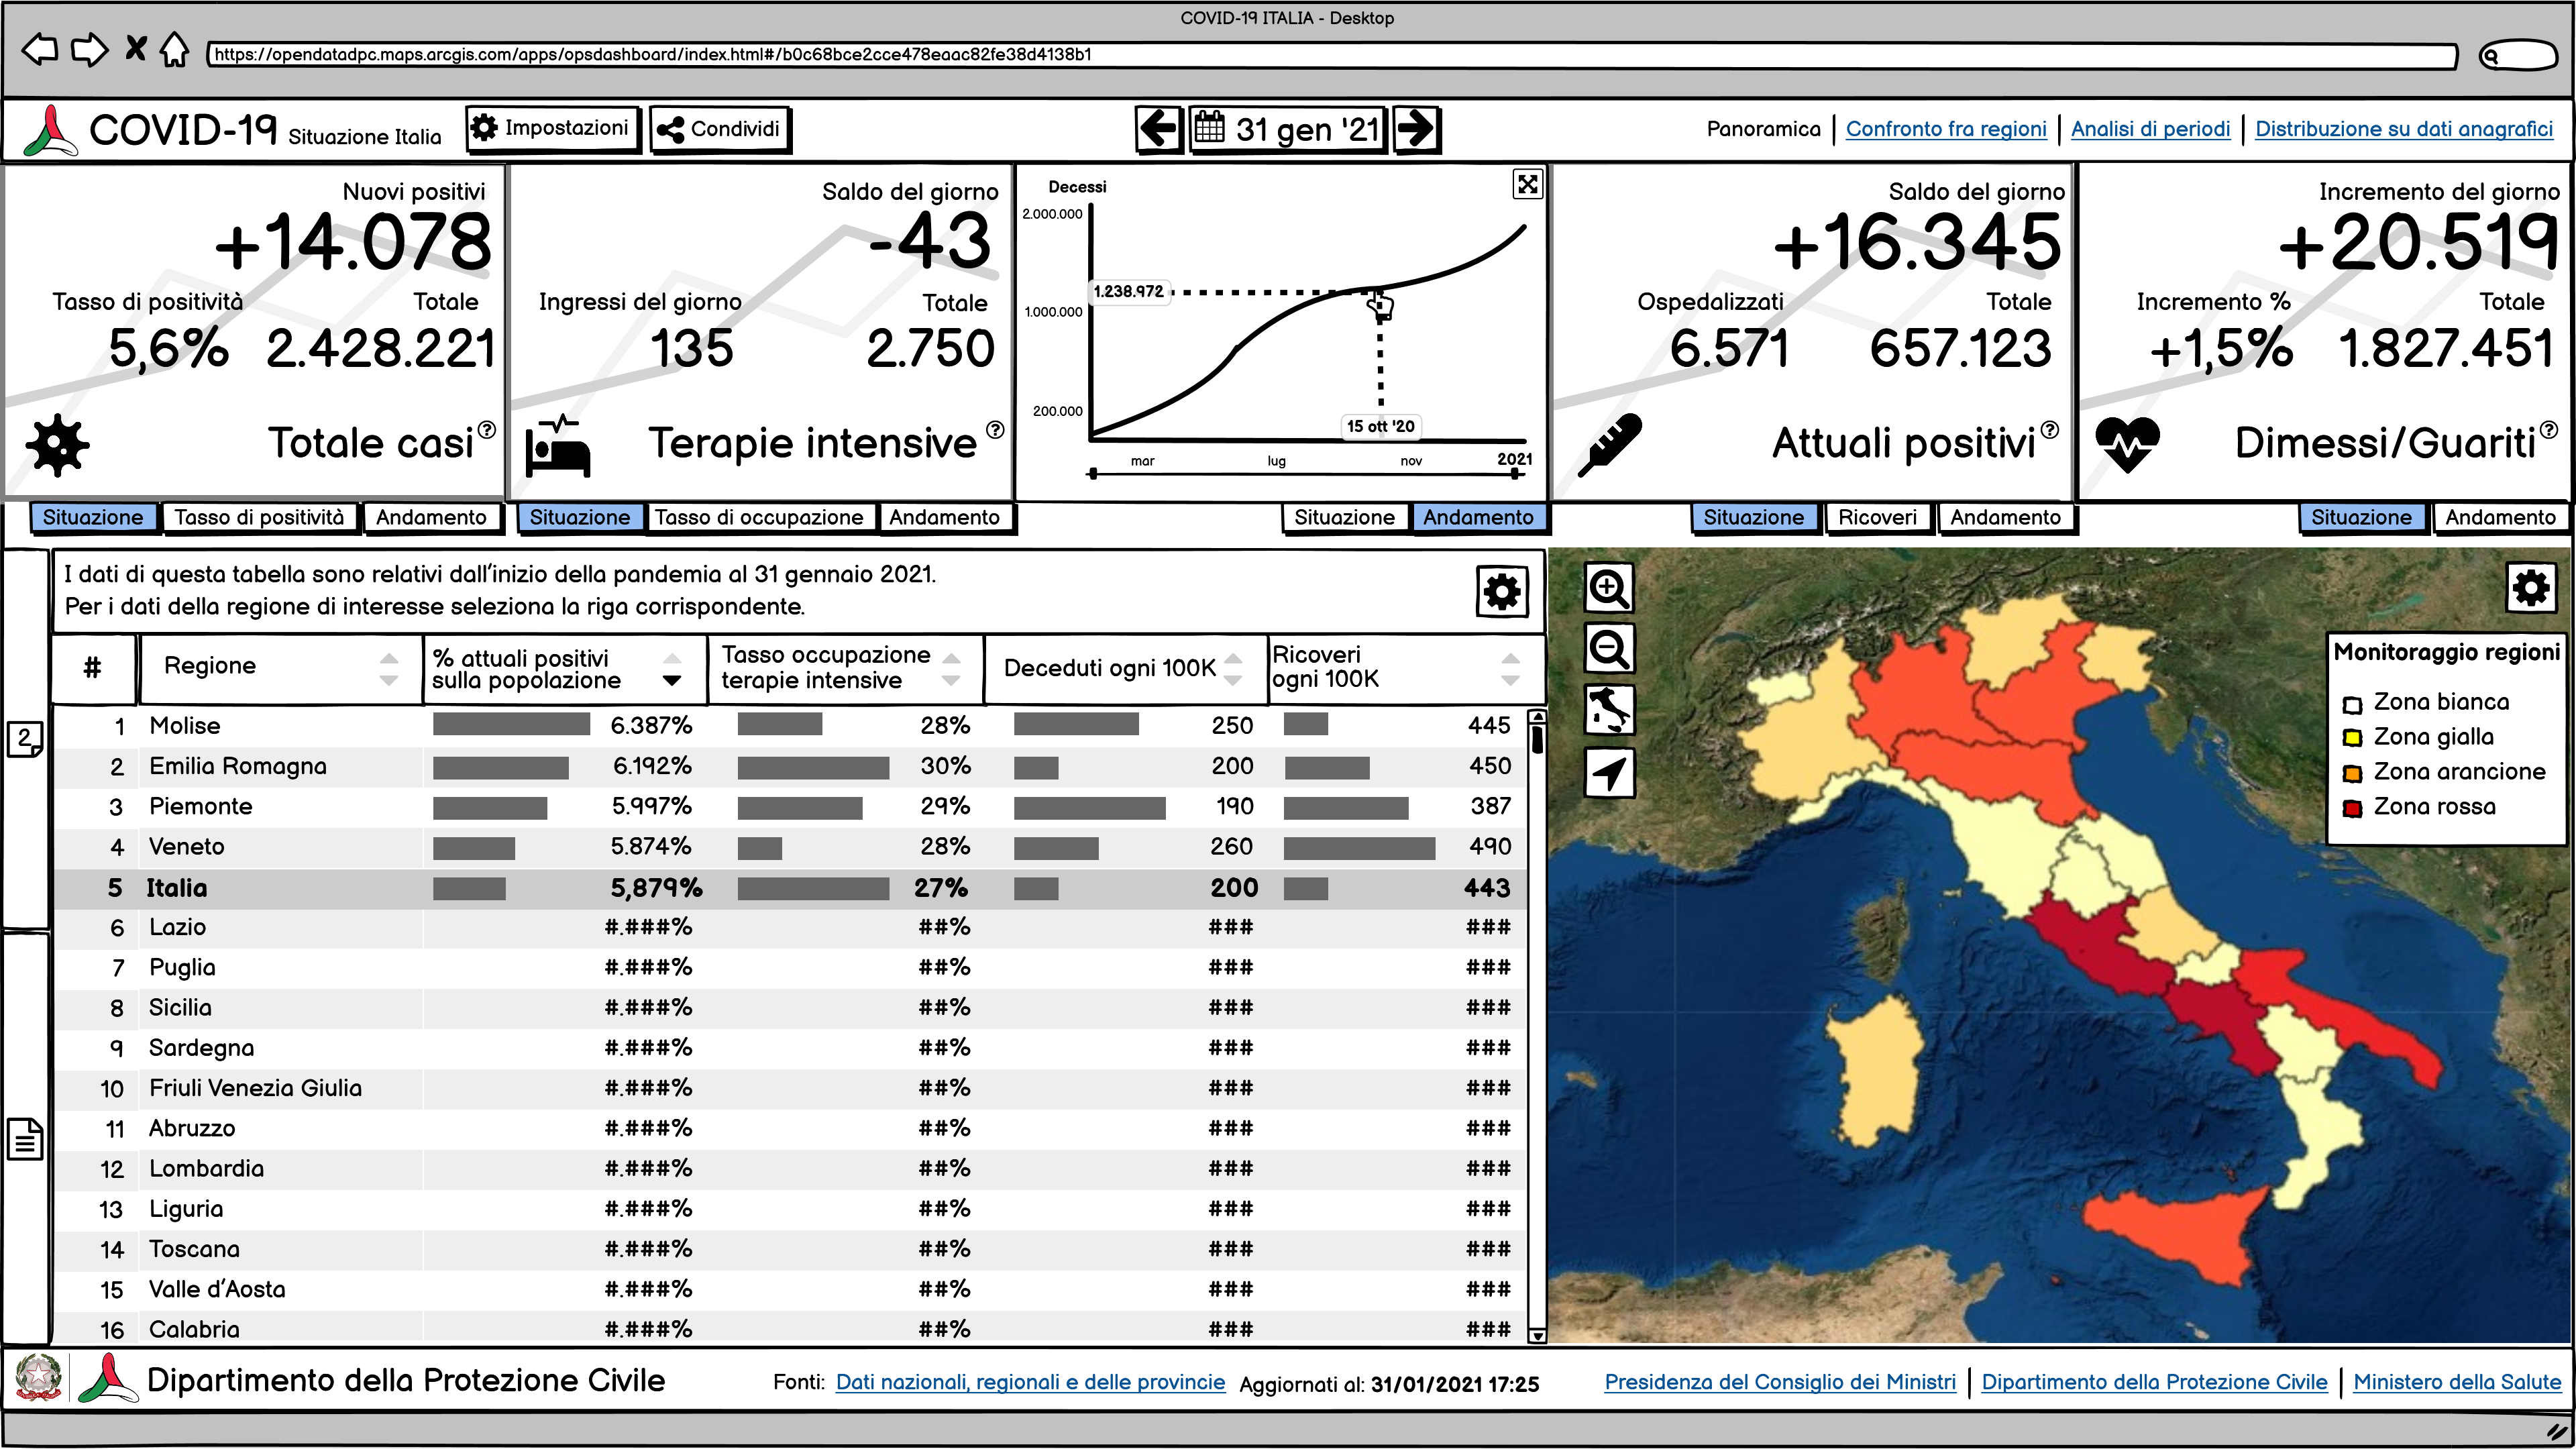
\includegraphics[trim=0 510 0 55, clip, width=.8\textwidth]{screen-interfaccia/6 - Panoramica.png}
        \caption{Parte alta della schermata "Panoramica" dell'interfaccia riprogettata.}
    \end{figure}

\end{frame}

\begin{frame}
    \frametitle{Panoramica - Tabella e mappa}
    Nella parte inferiore, vi è una tabella che presenta i dati epidemiologici per le regioni italiane; ancora, vi è una heat map che offre un efficace colpo d'occhio circa la distribuzione della metrica selezionata sul territorio nazionale. 
    \begin{figure}
        \centering
        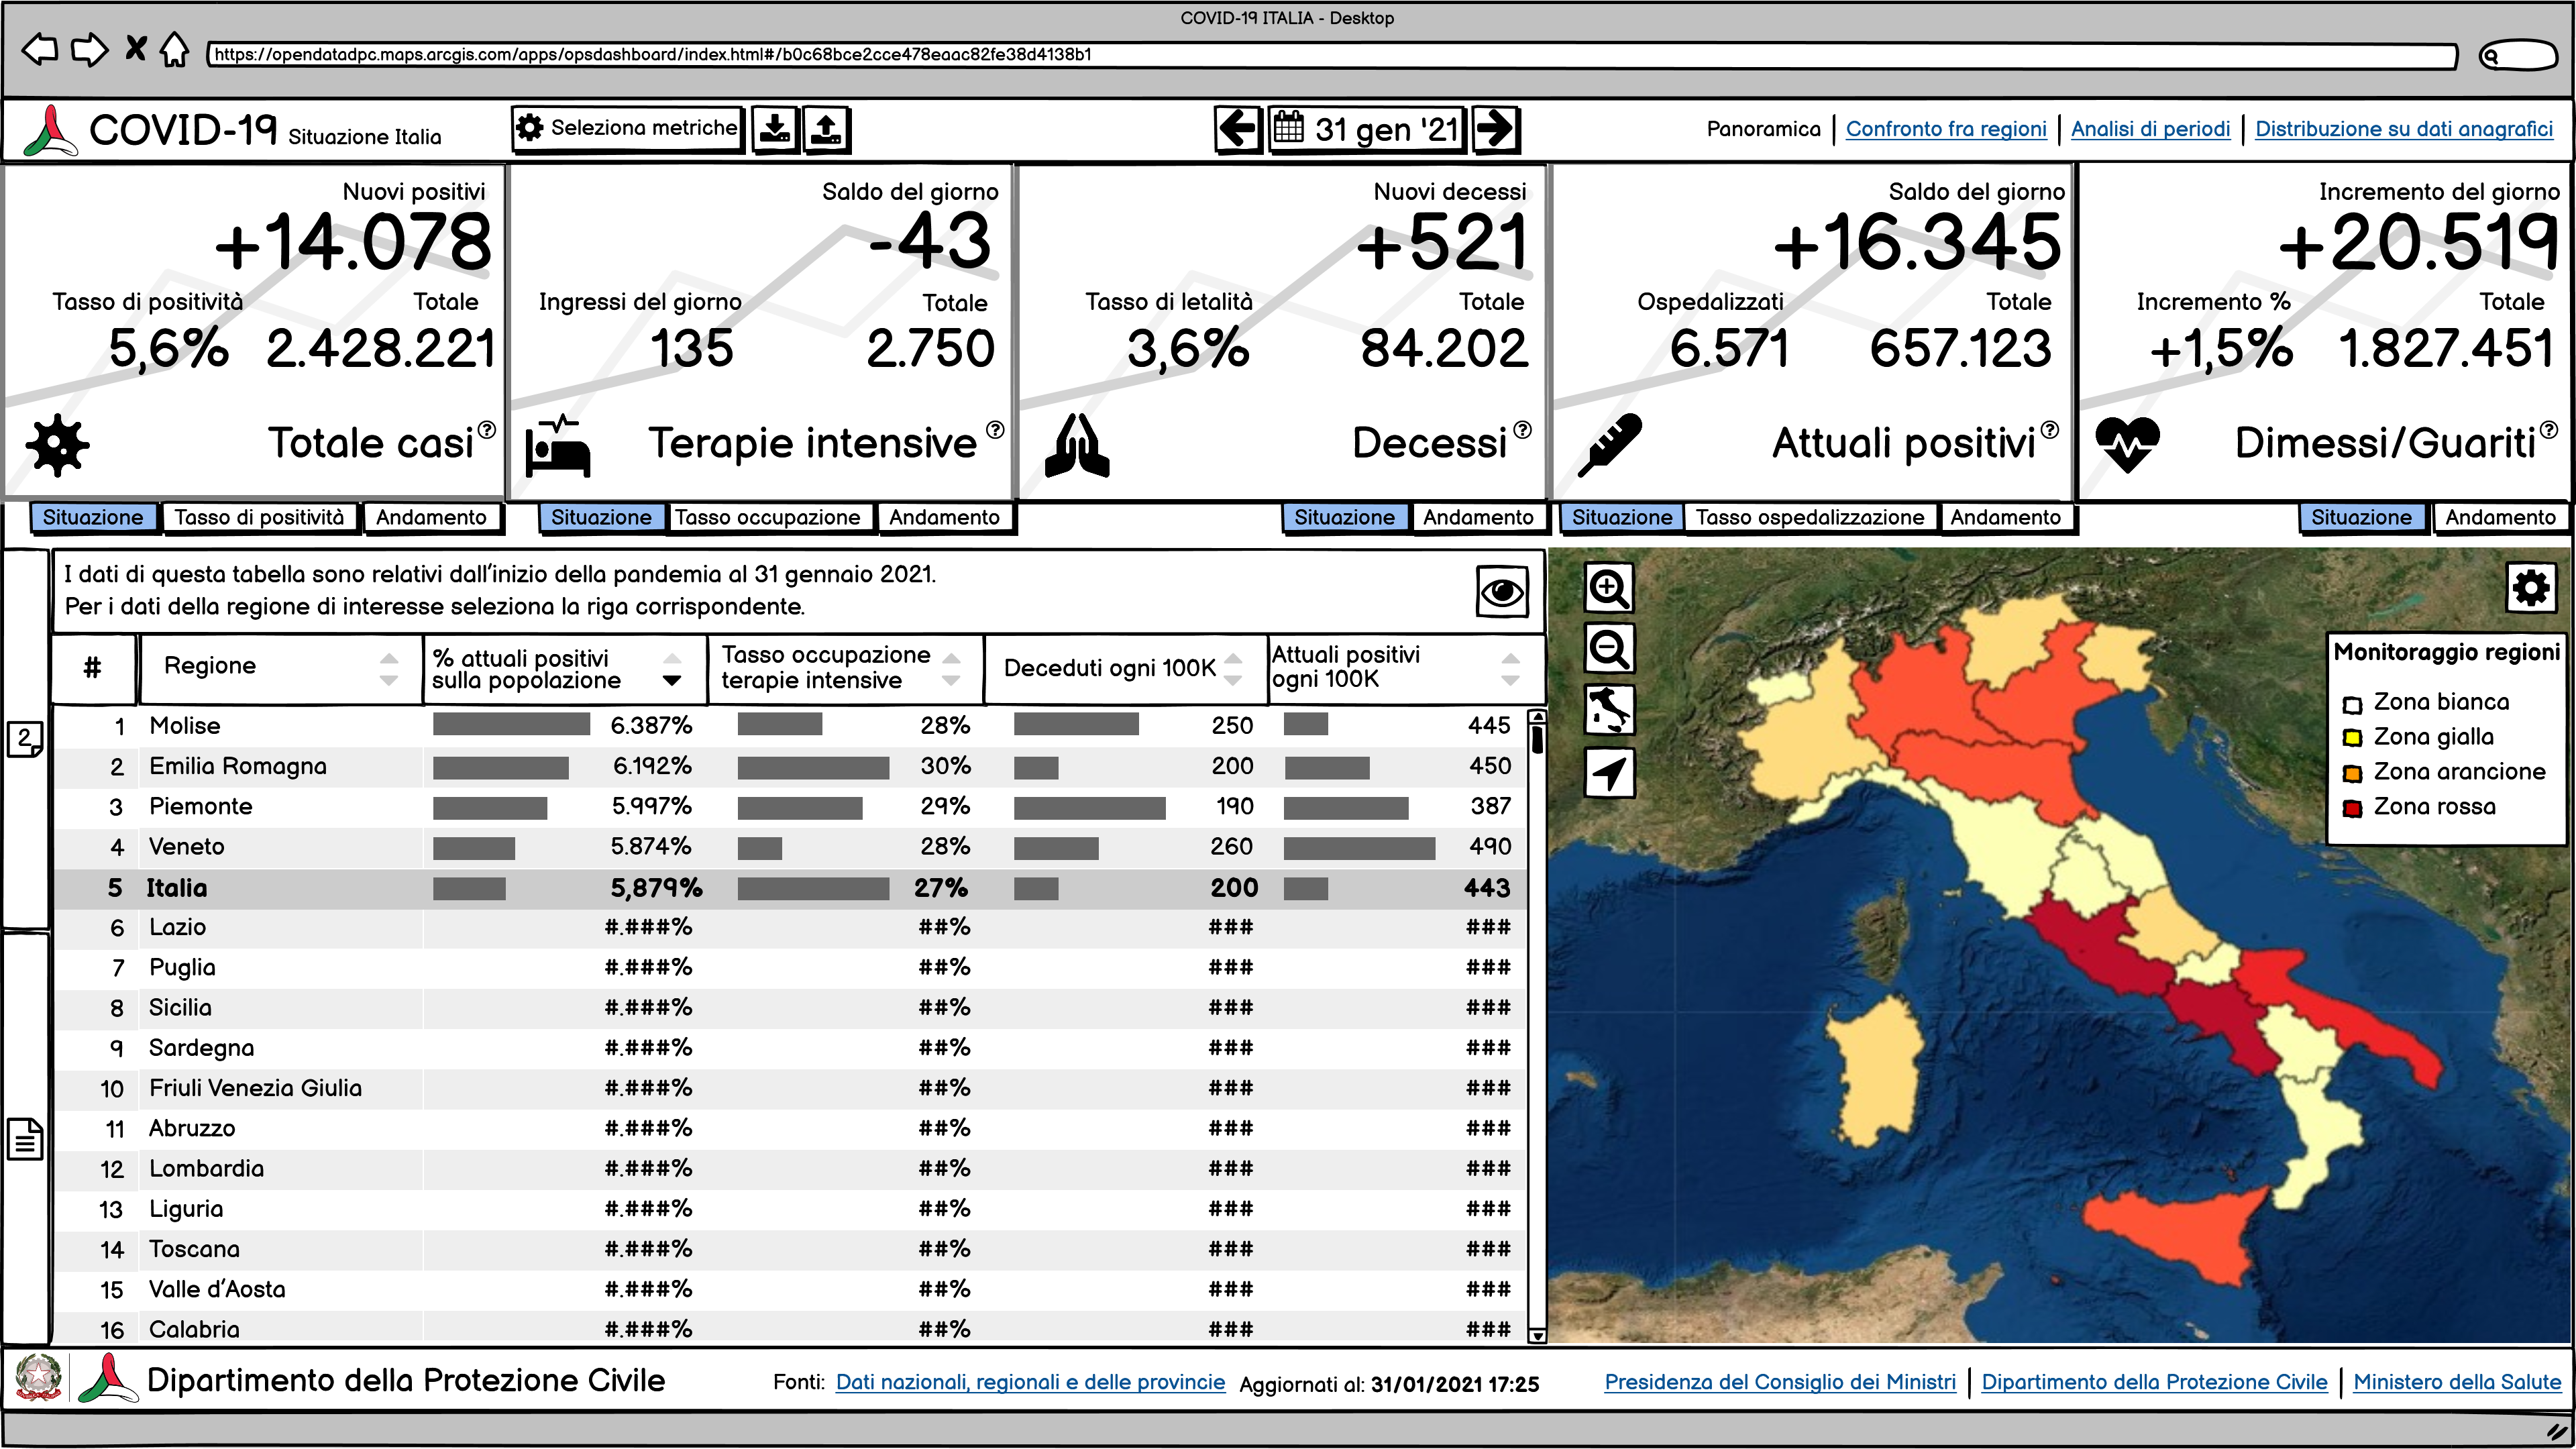
\includegraphics[trim=0 20 0 305, clip, width=.8\textwidth]{screen-interfaccia/1 - Panoramica.png}
        \caption{Parte bassa della schermata "Panoramica" dell'interfaccia riprogettata.}
    \end{figure}
    \vspace{-10pt}
    Per i dati di una regione, cliccarne l'area nella mappa o la riga nella tabella.

\end{frame}

\begin{frame}
    \frametitle{Confronto tra regioni}
    \label{confronto-regioni}
    Per selezionare le regioni che si vogliono confrontare, è sufficiente cliccarne l'area sulla mappa o sceglierle nell'elenco a discesa soprastante.
    \begin{figure}
        \centering
        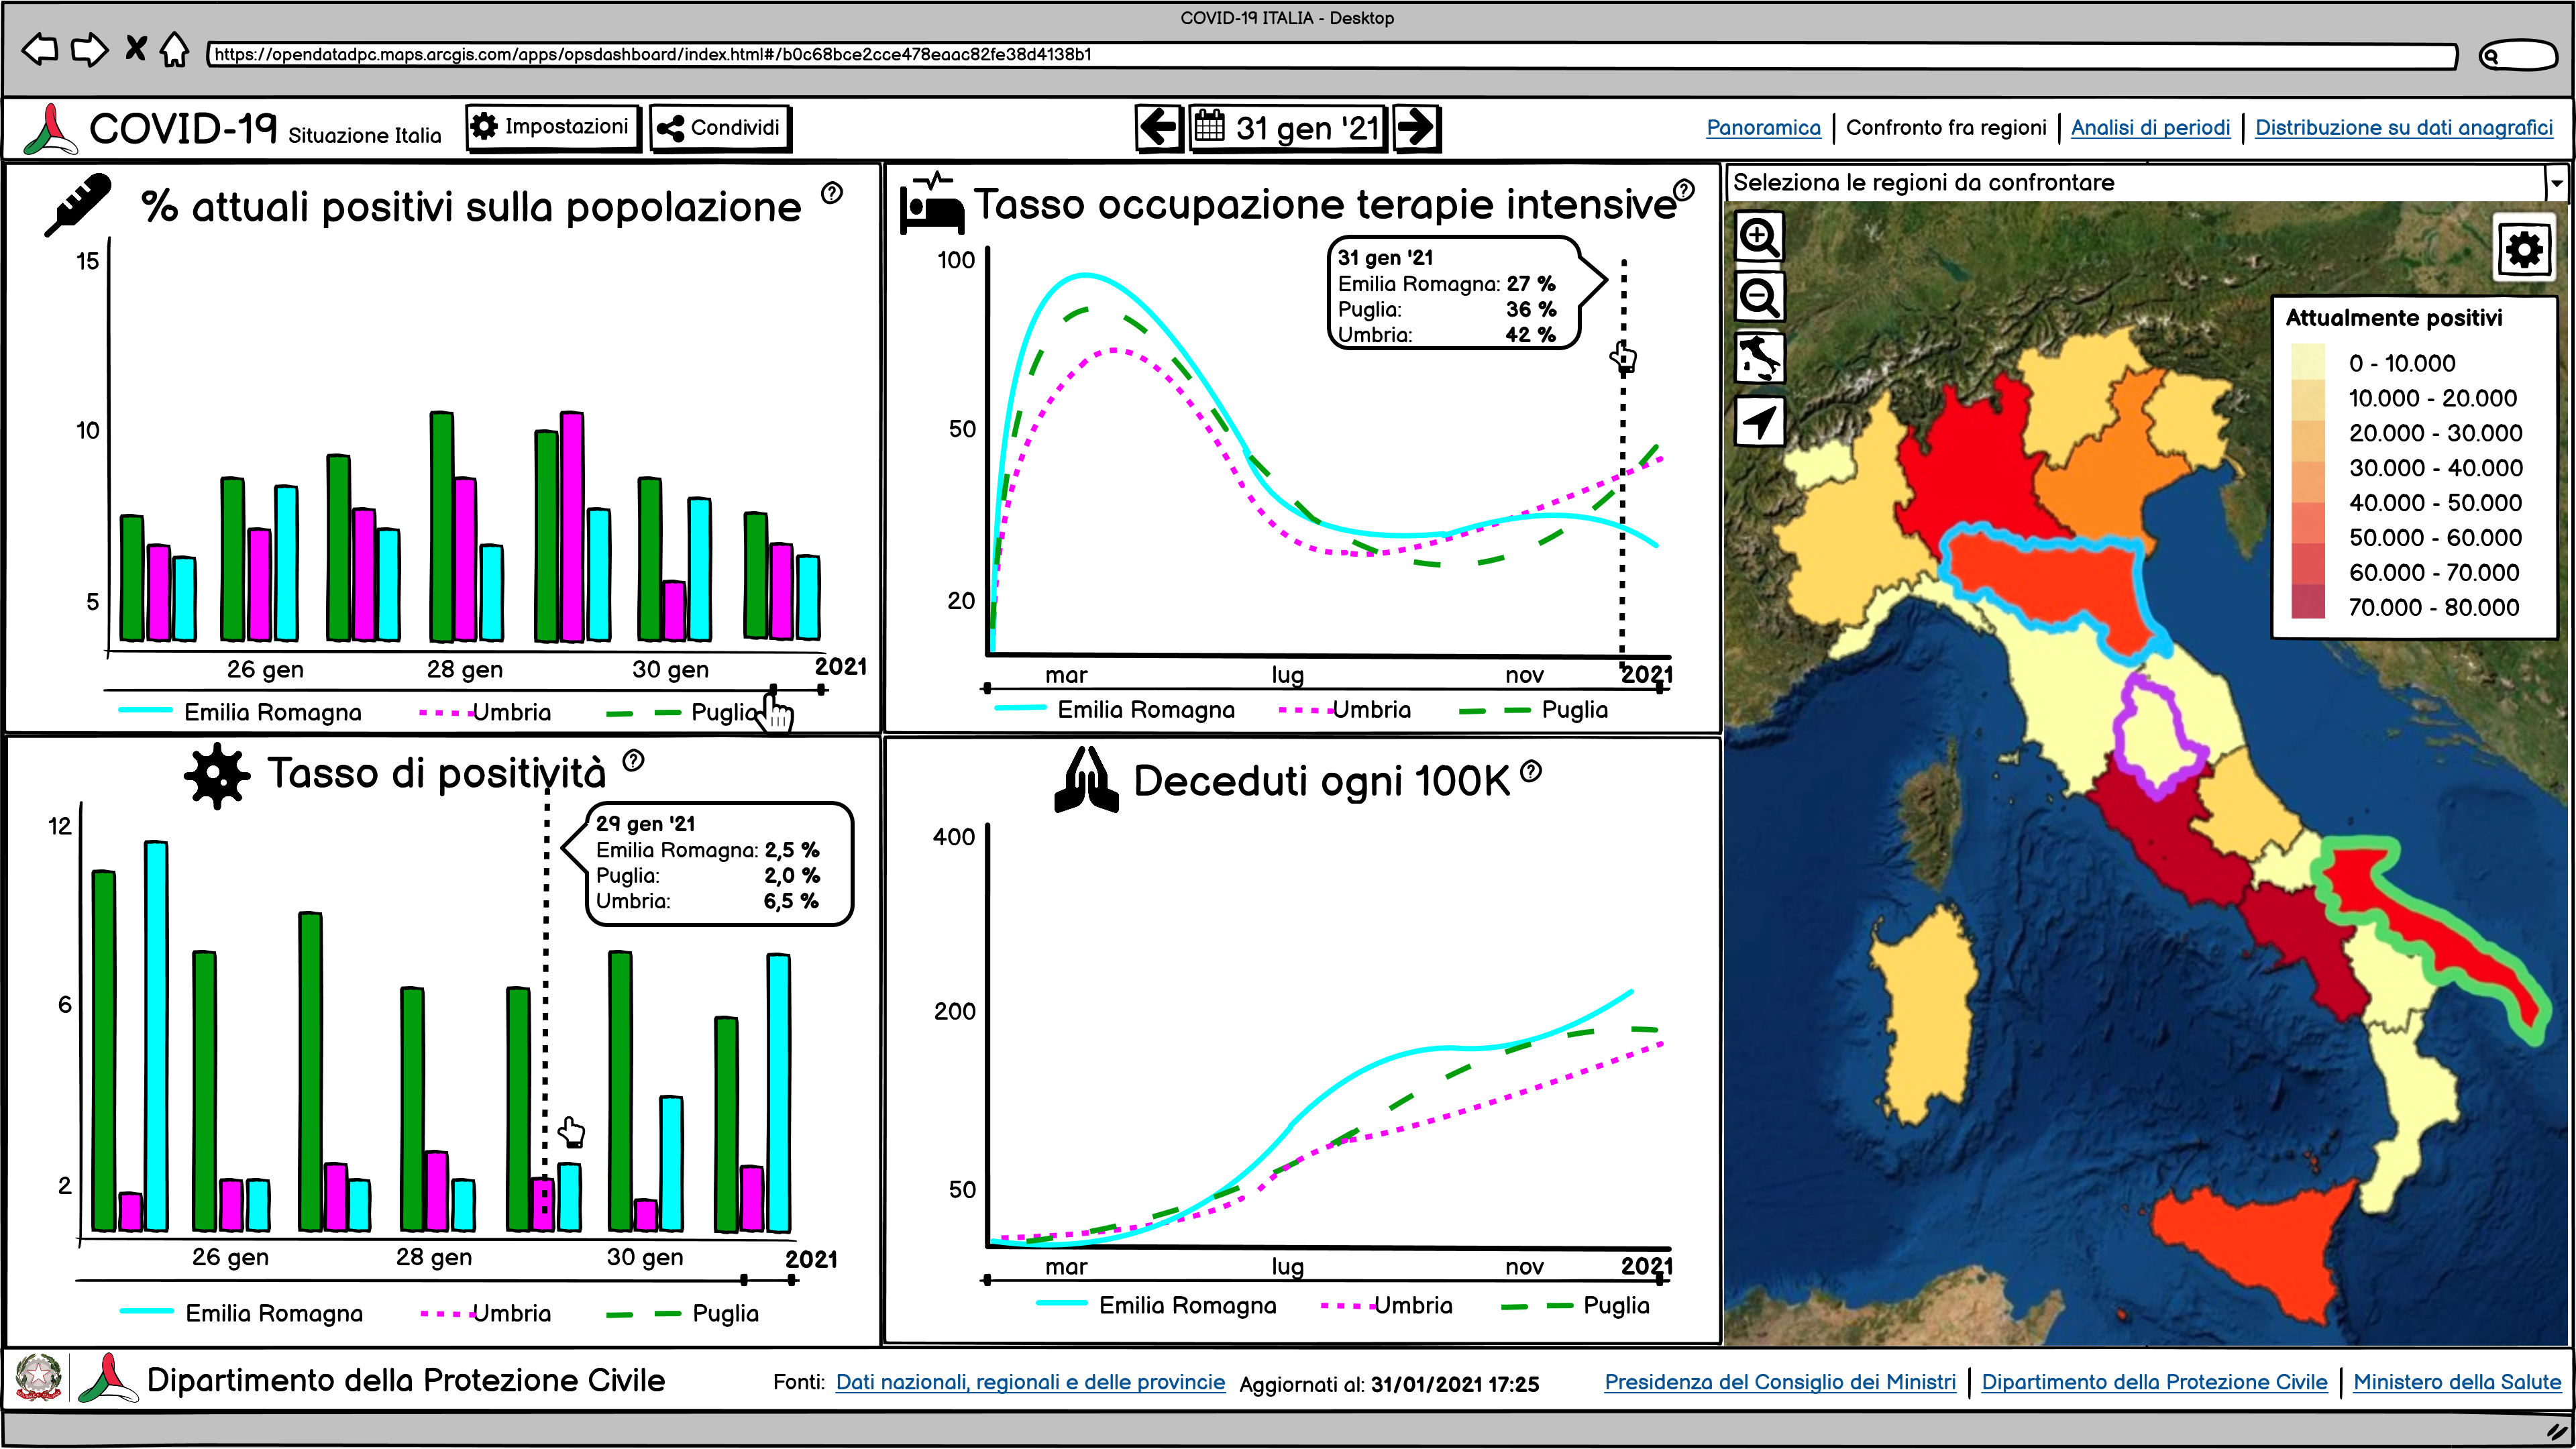
\includegraphics[width=.6\textwidth]{screen-interfaccia/1 - Confronto fra regioni}
        \caption{Schermata "Confronto tra regioni" dell'interfaccia riprogettata.}
    \end{figure}    

\end{frame}


\begin{frame}
    \frametitle{Analisi di periodi}
    \label{analisi-periodi}
    \begin{figure}
        \centering
        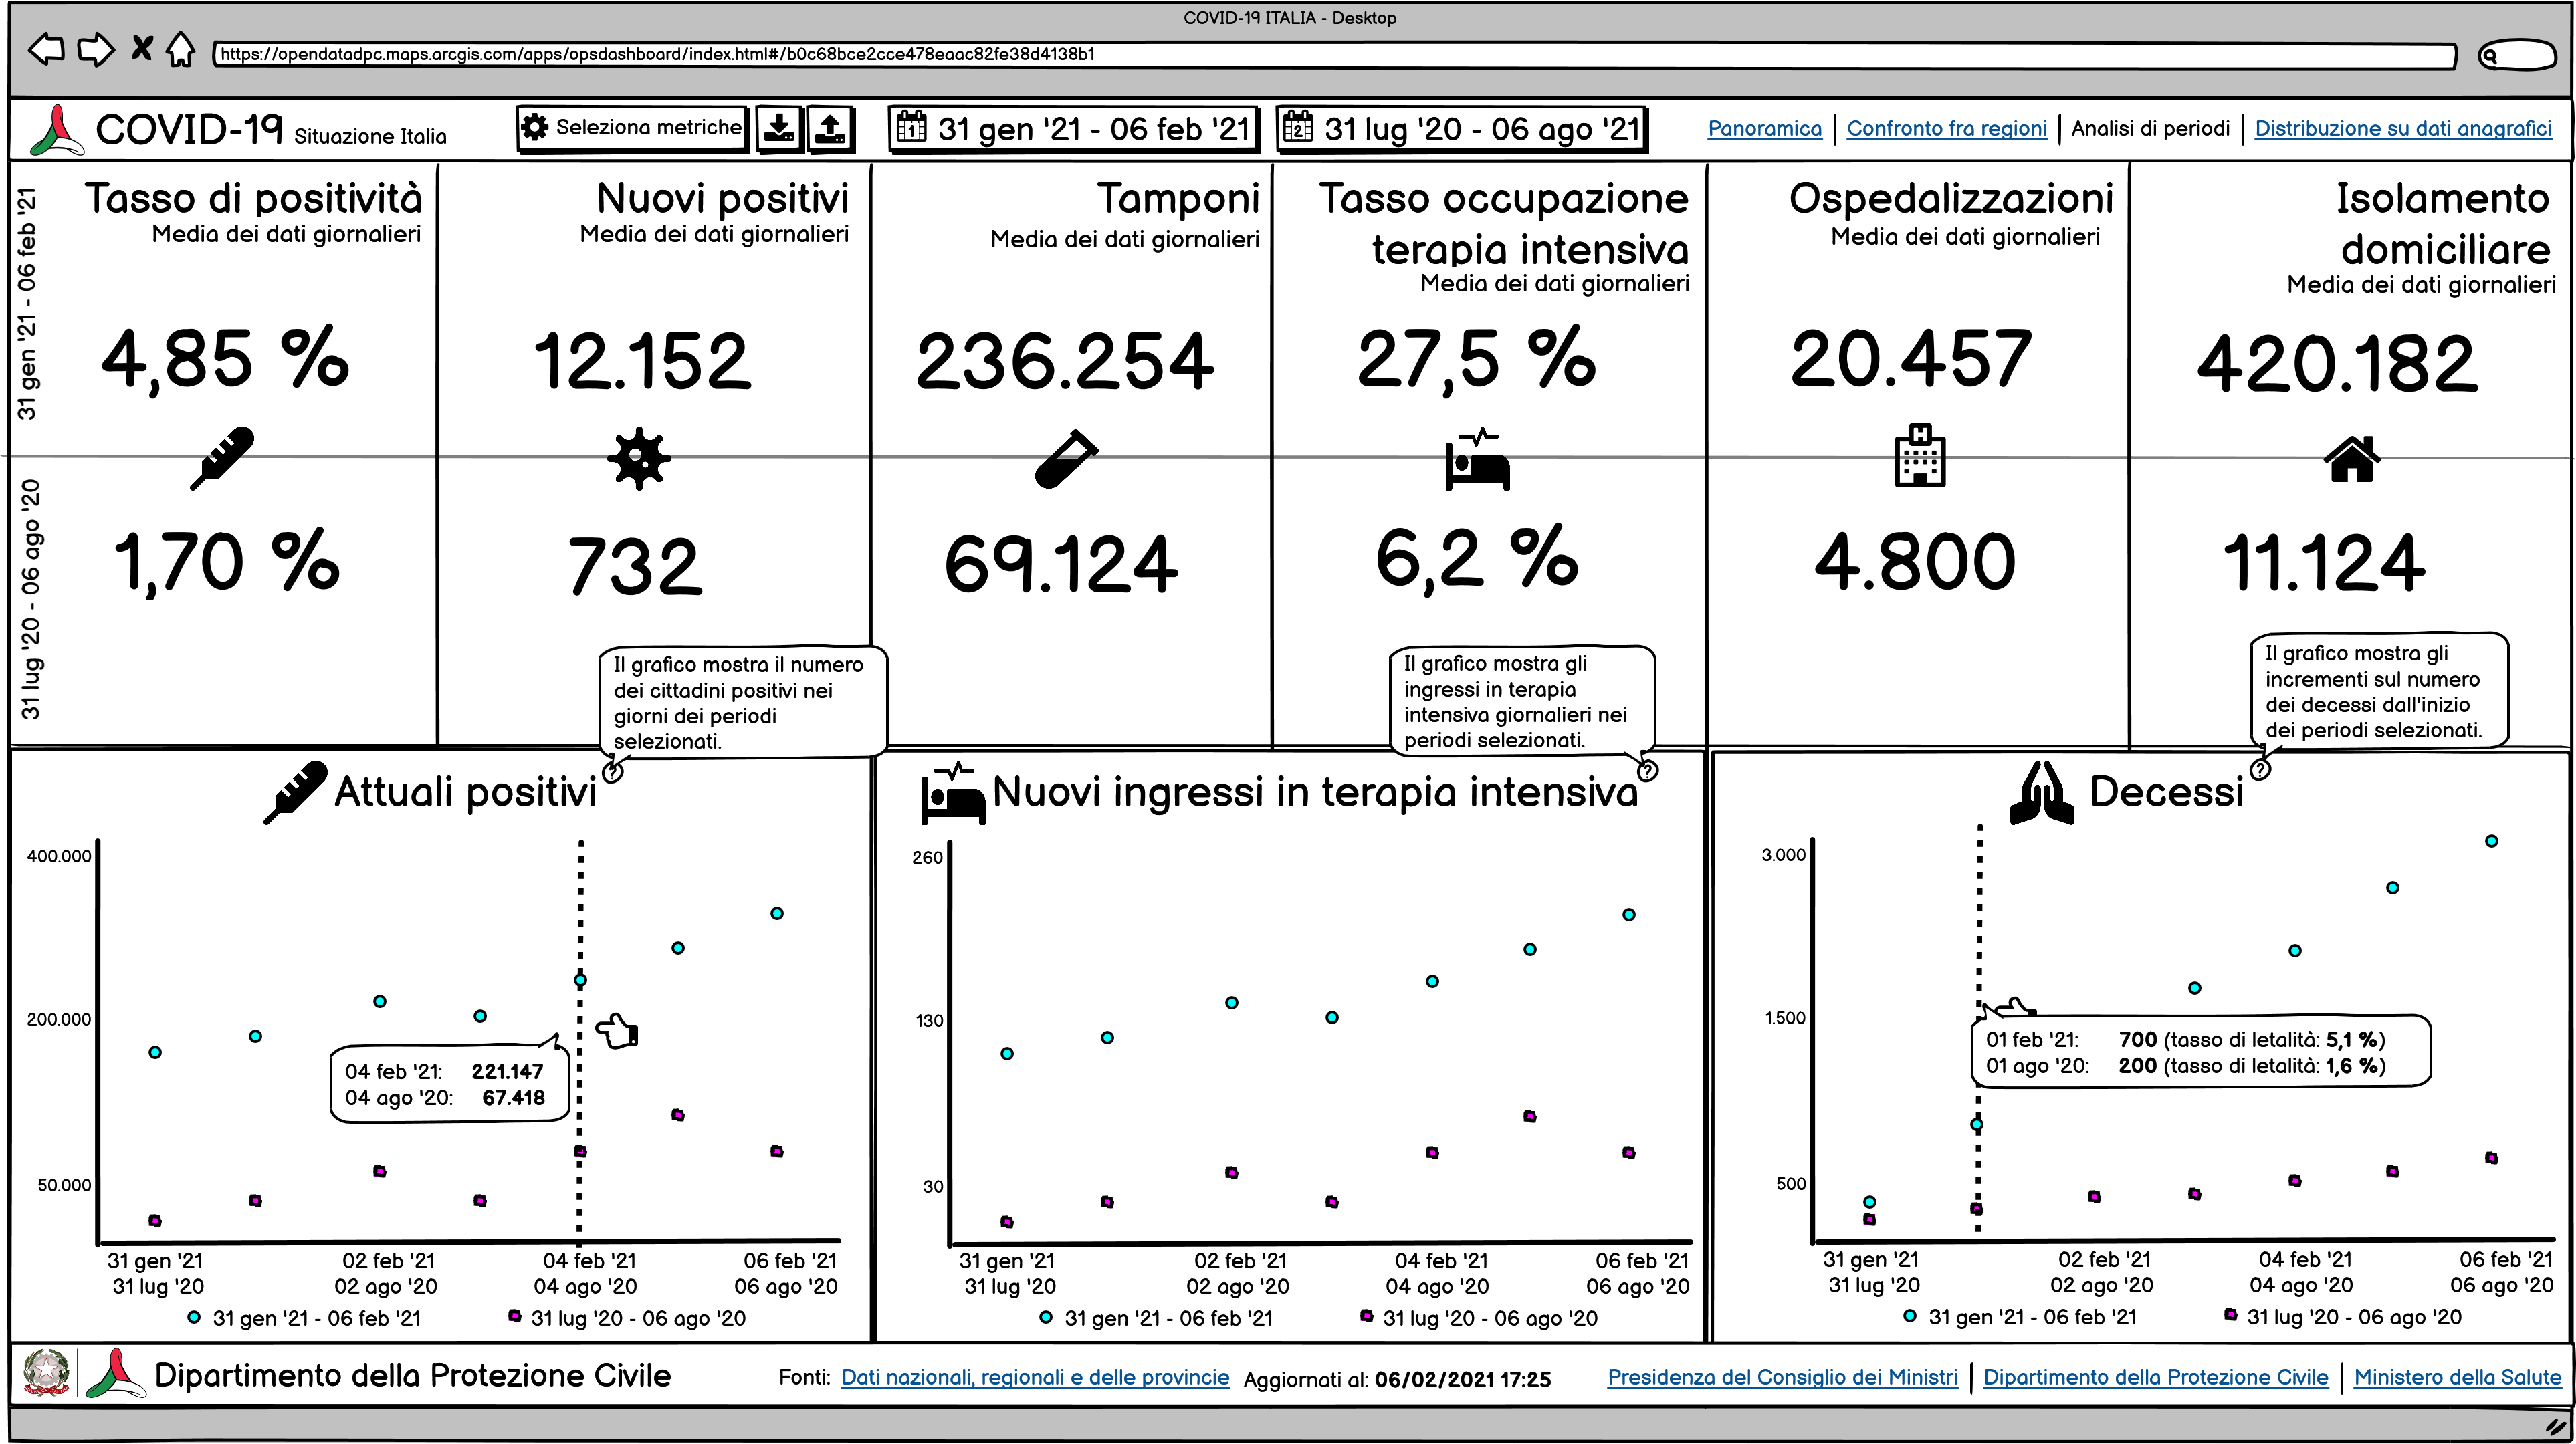
\includegraphics[width=.7\textwidth]{screen-interfaccia/1 - Analisi di periodi}
        \caption{Schermata "Analisi di periodi" dell'interfaccia riprogettata.}
    \end{figure}    

\end{frame}

\begin{frame}
    \frametitle{Analisi di periodi - Box}
    Nella parte superiore, sono visualizzati i valori delle metriche aggregati sul o sui periodi temporali specificati, permettendo al giornalista di raffrontare immediatamente i valori stessi.
    \begin{figure}
        \centering
        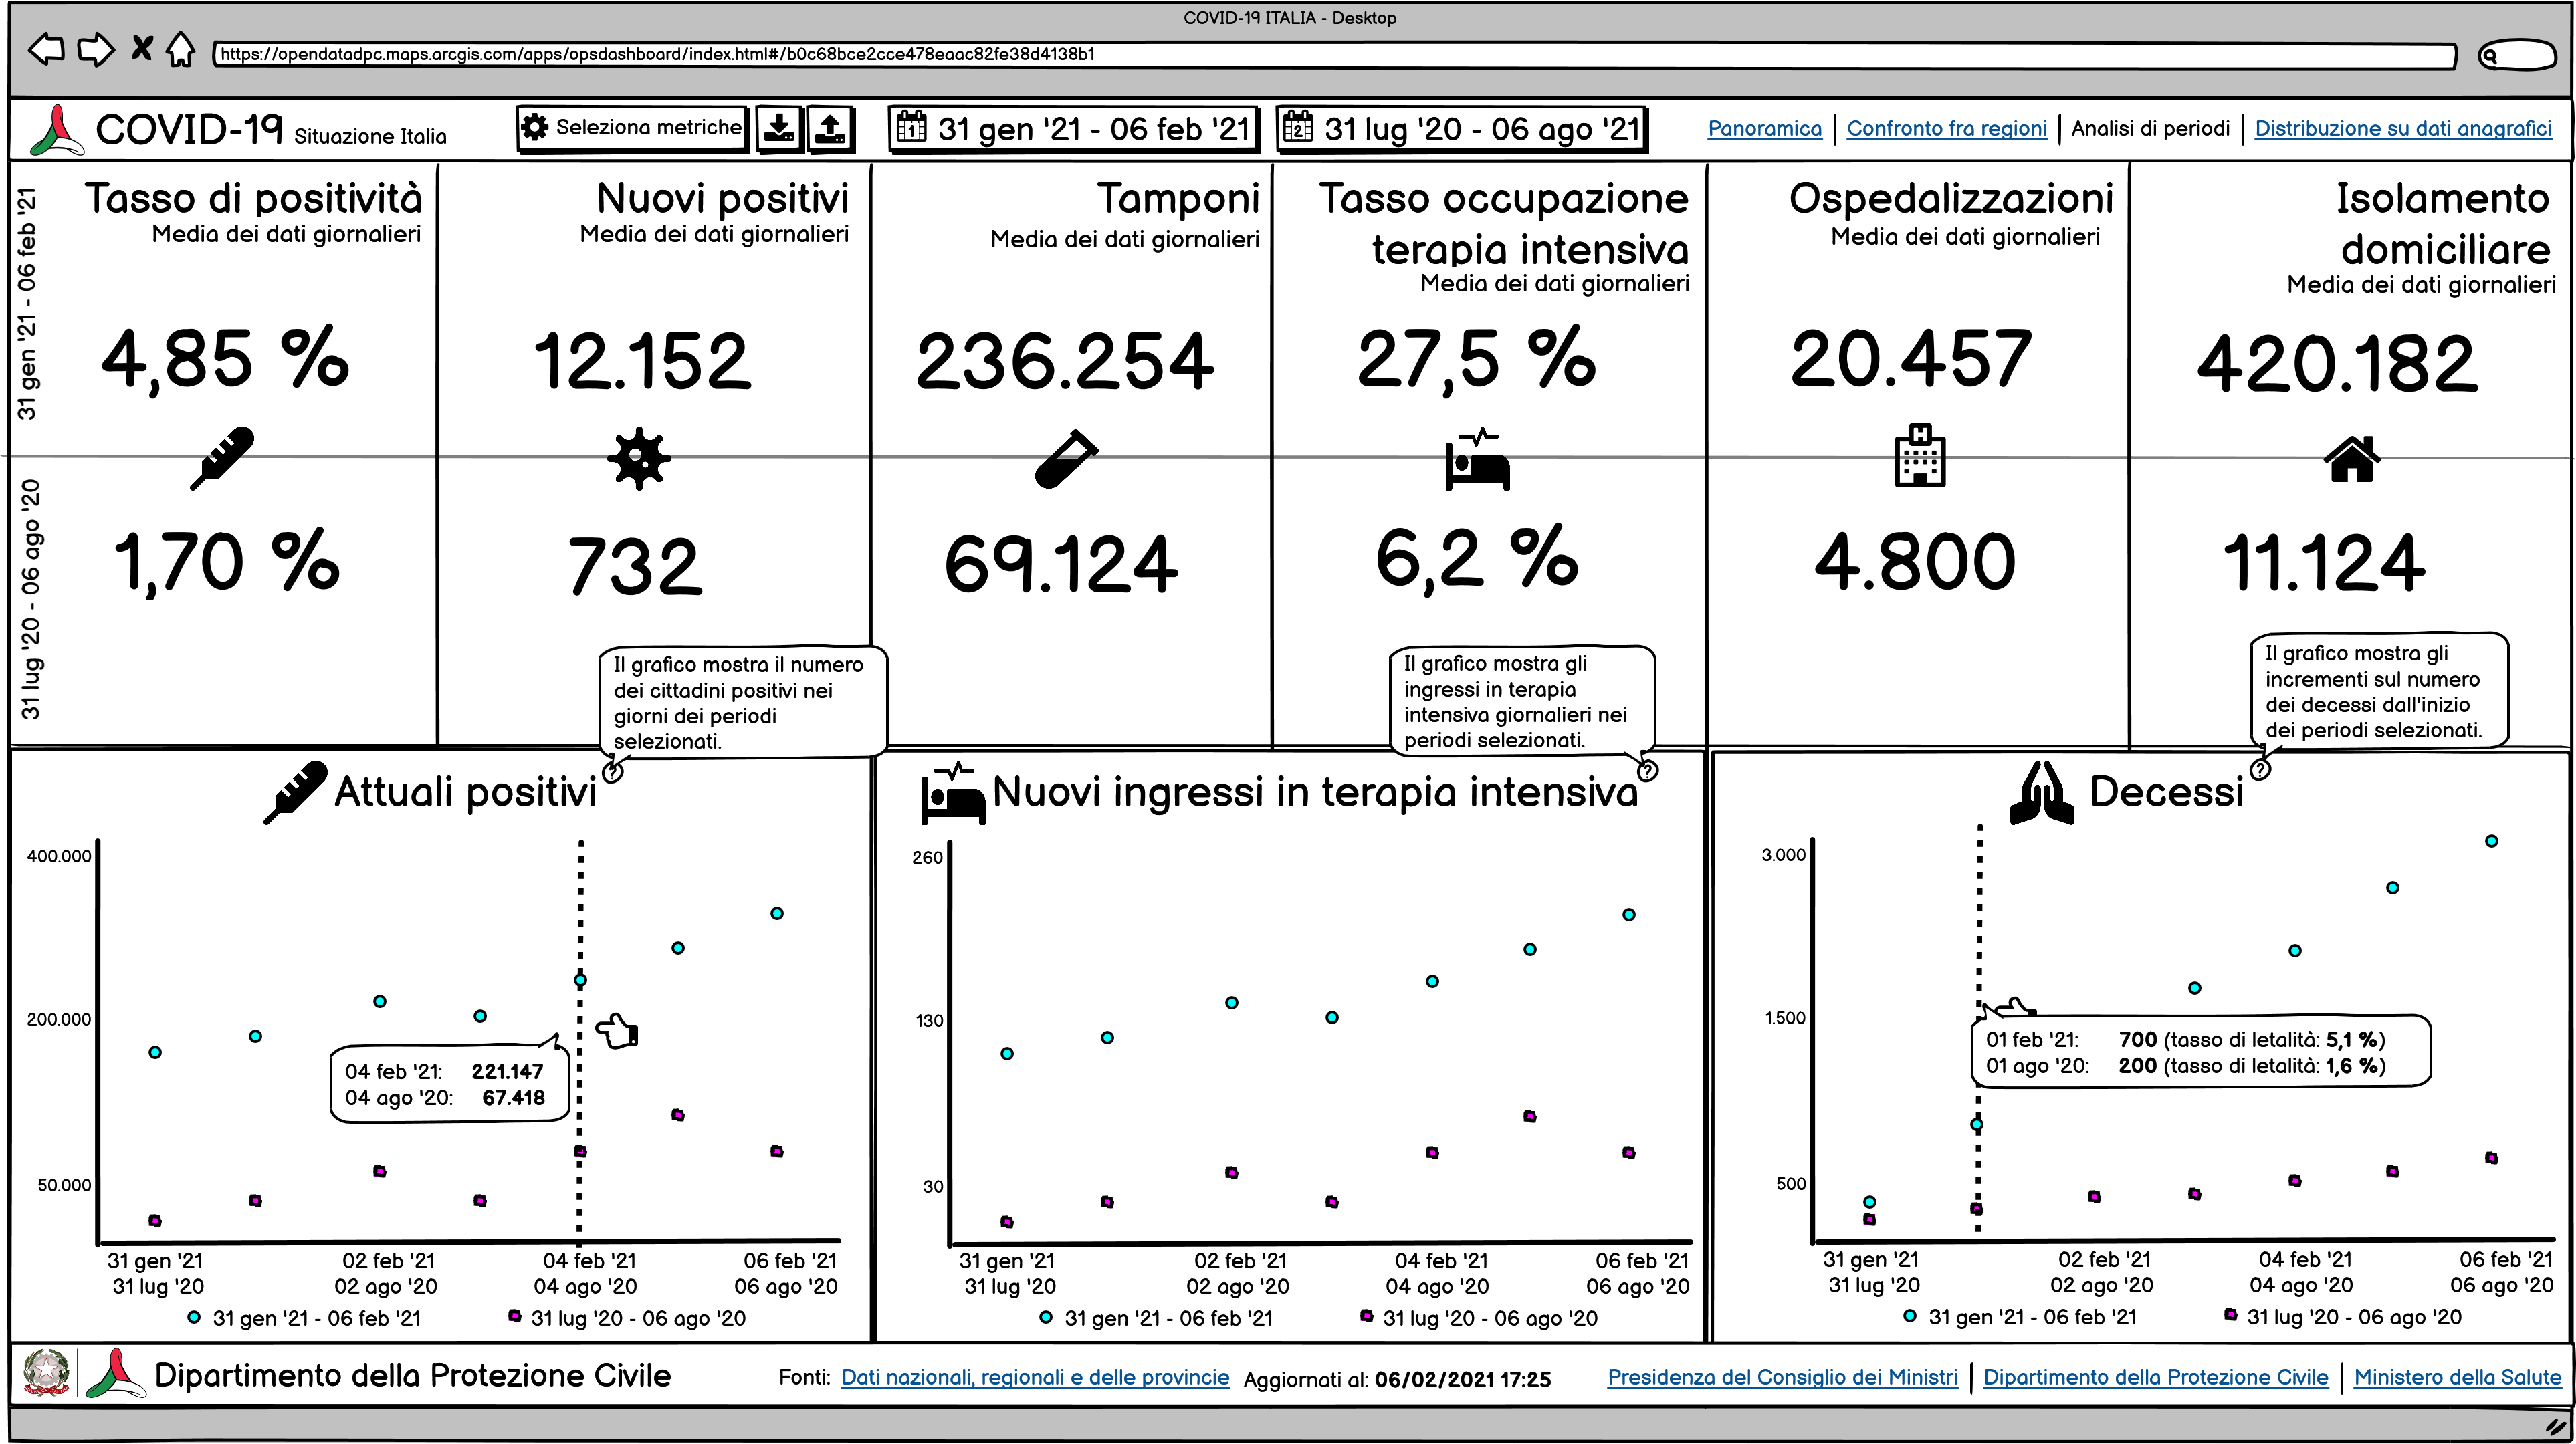
\includegraphics[trim=0 400 0 55, clip, width=.7\textwidth]{screen-interfaccia/1 - Analisi di periodi}
        \caption{Parte alta della schermata "Analisi di periodi" dell'interfaccia riprogettata.}
    \end{figure}    

\end{frame}

\begin{frame}
    \frametitle{Analisi di periodi - Grafici}
    Nella parte inferiore, trovano spazio tre grafici che riportano gli andamenti delle metriche relativamente alla o alle finestre temporali fissate.
    \vspace{20pt}
    \begin{figure}
        \centering
        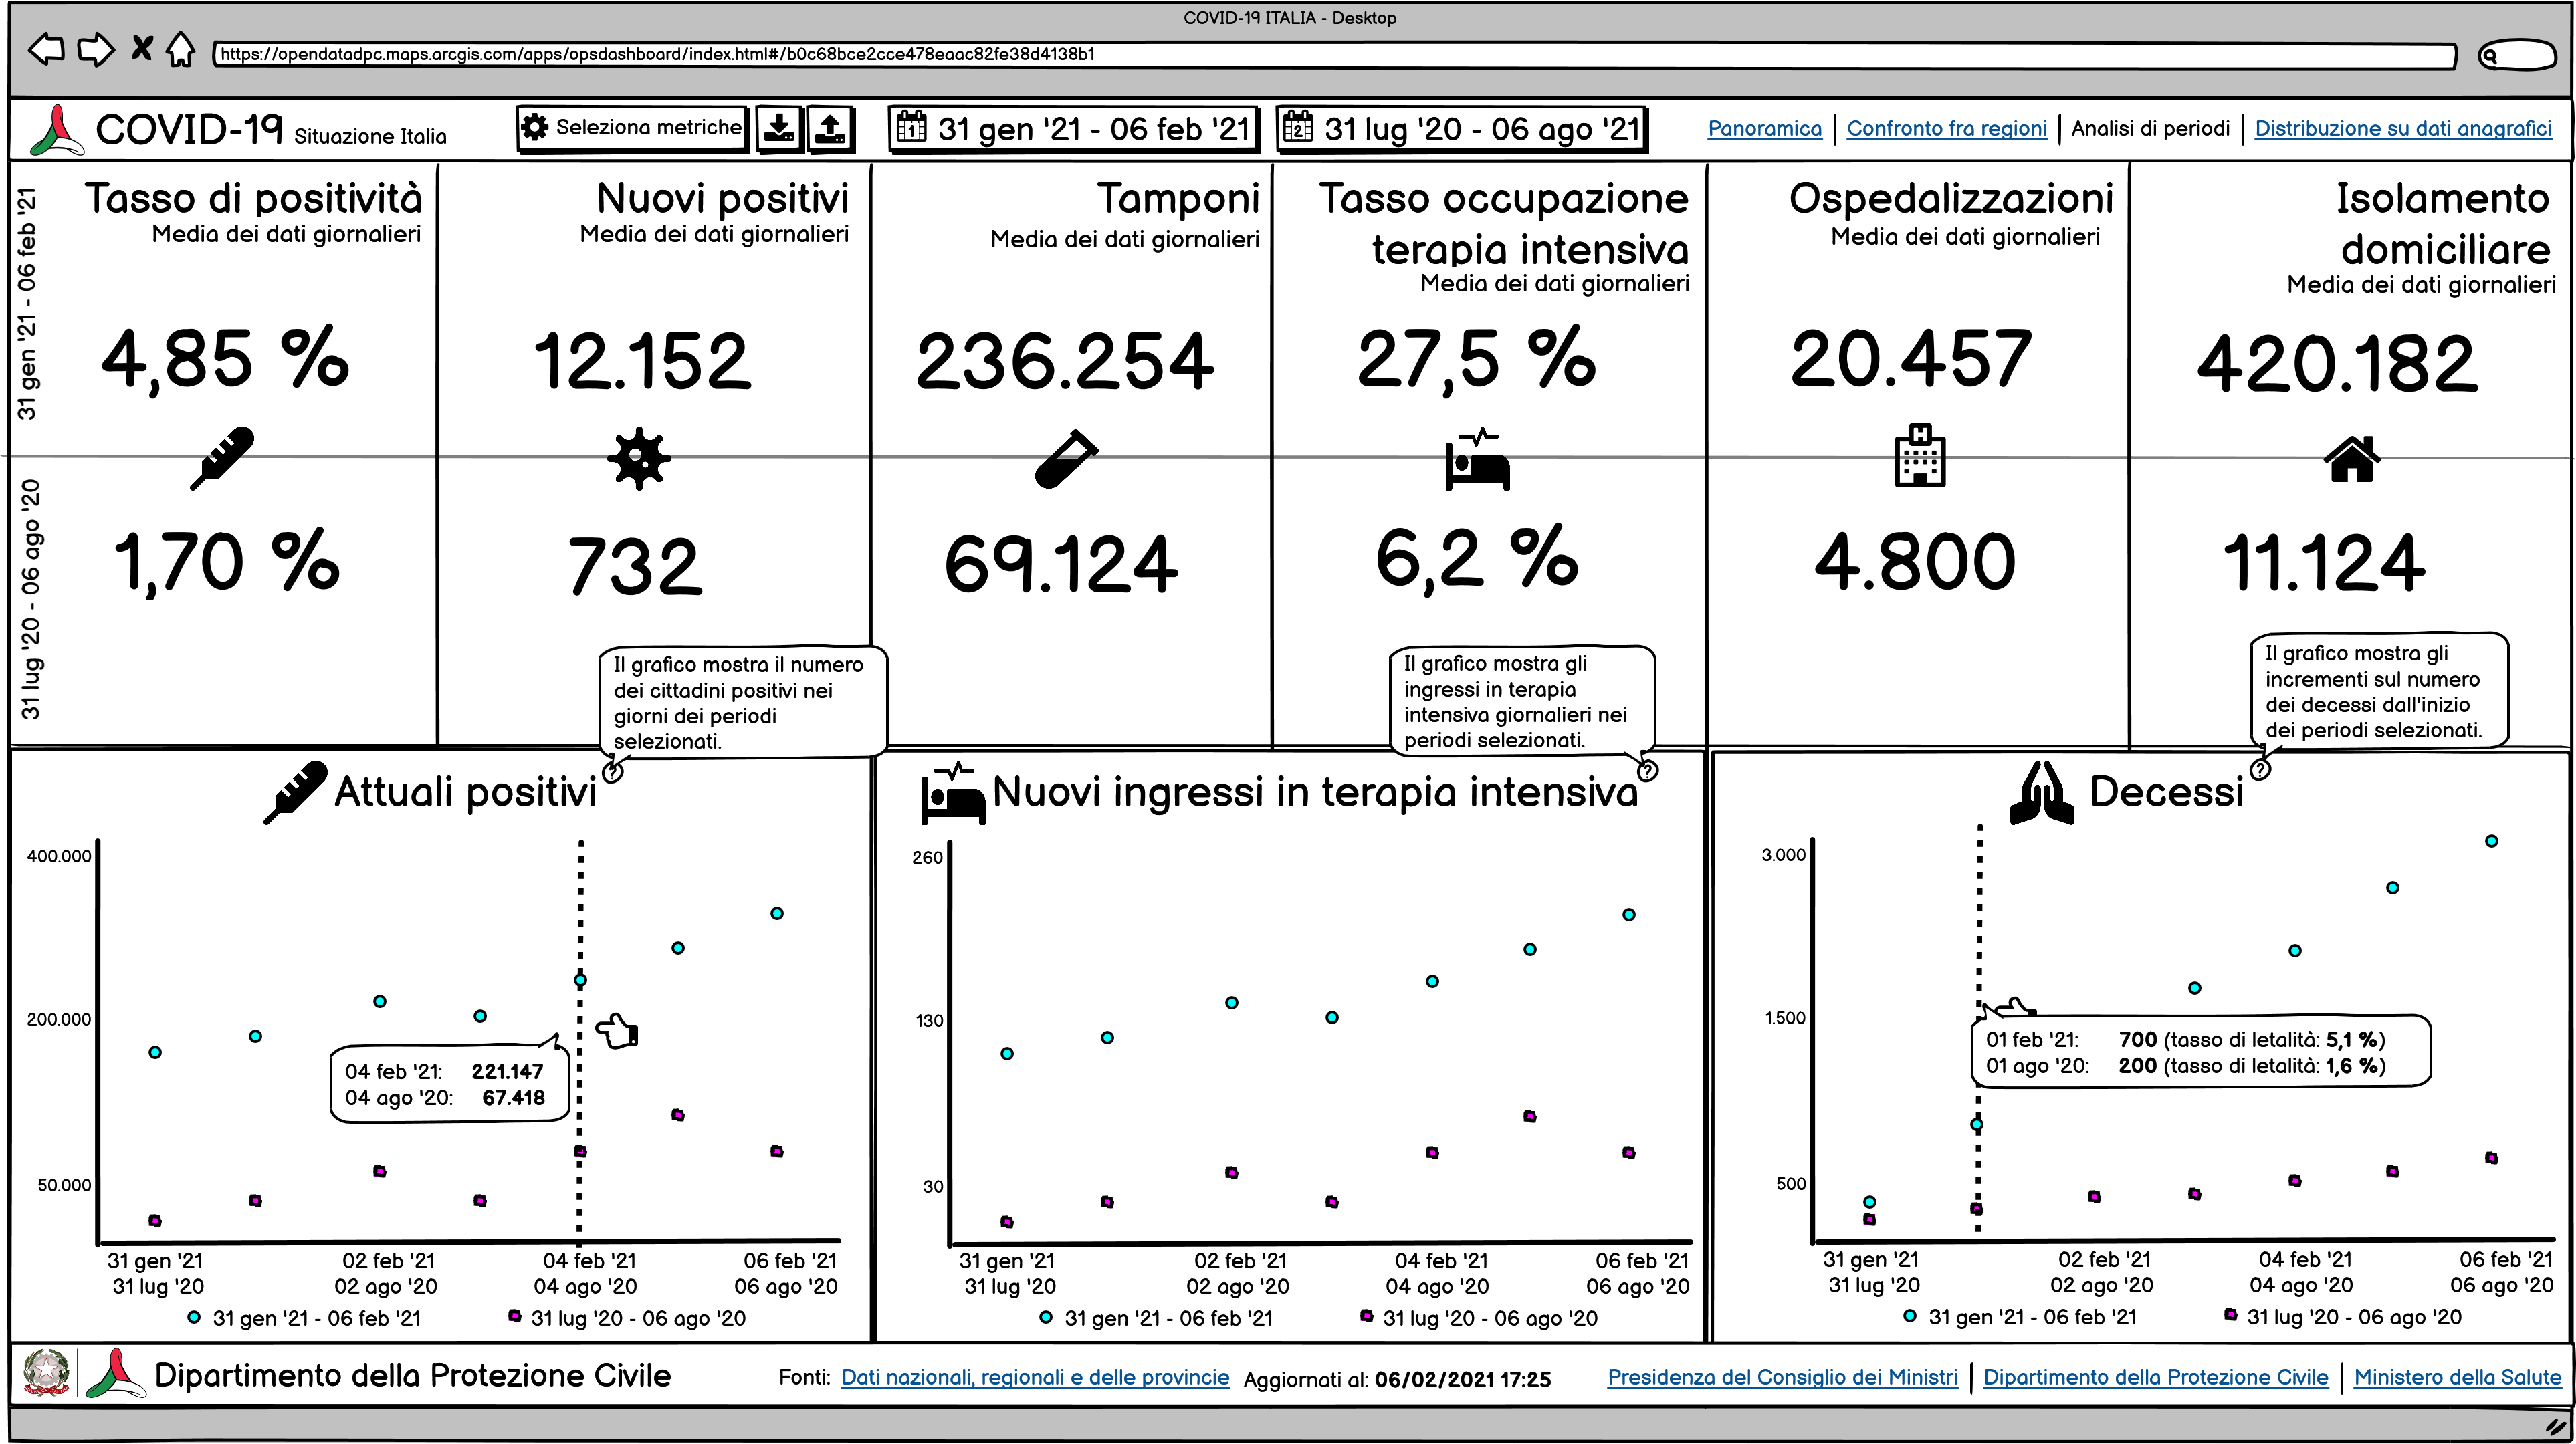
\includegraphics[trim=0 20 0 420, clip, width=.7\textwidth]{screen-interfaccia/1 - Analisi di periodi}
        \caption{Parte bassa della schermata "Analisi di periodi" dell'interfaccia riprogettata.}
    \end{figure}    

\end{frame}

\begin{frame}
    \frametitle{Distribuzione sui dati anagrafici}
    \label{distribuzione}
    \begin{figure}
        \centering
        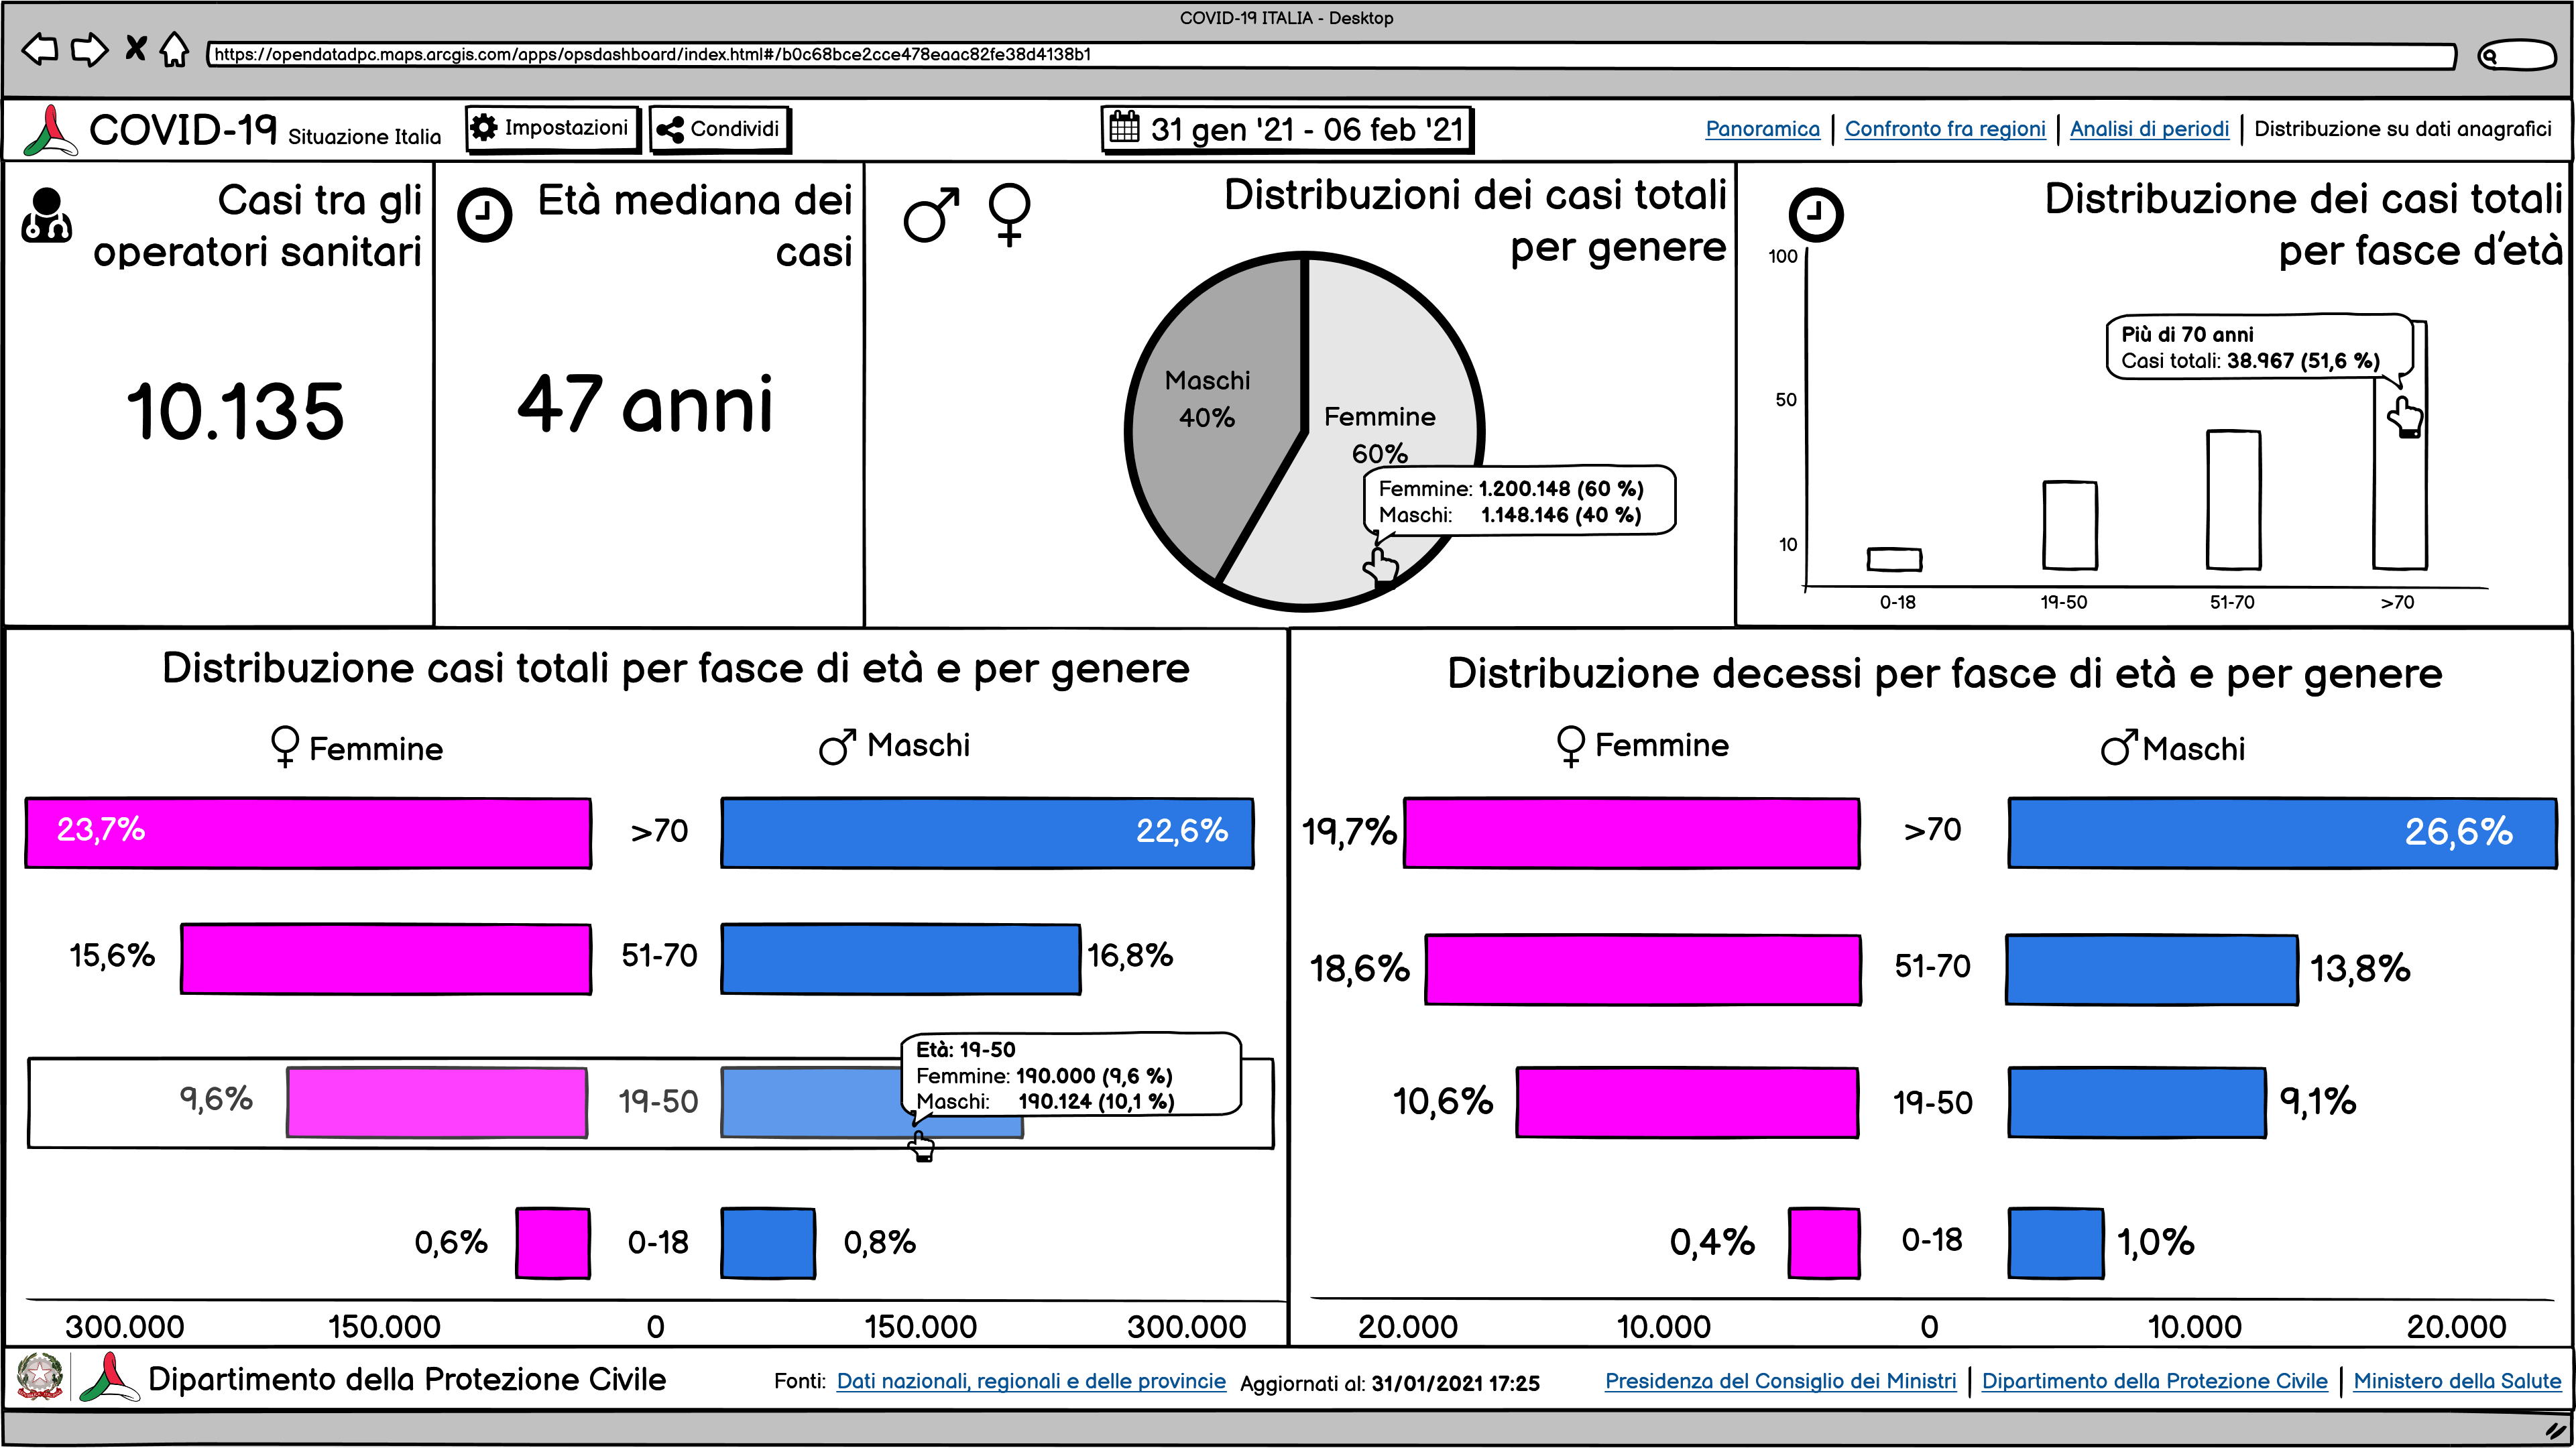
\includegraphics[width=.7\textwidth]{screen-interfaccia/1 - Distribuzione su dati anagrafici}
        \caption{Schermata "Distribuzione su dati anagrafici" dell'interfaccia riprogettata.}
    \end{figure}    

\end{frame}

\begin{frame}
    \frametitle{Distr. sui dati anagrafici - Distr. semplici}
    Nella parte alta, sono mostrate distribuzioni semplici per età o per genere.
    \begin{figure}
        \centering
        \vspace{20pt}
        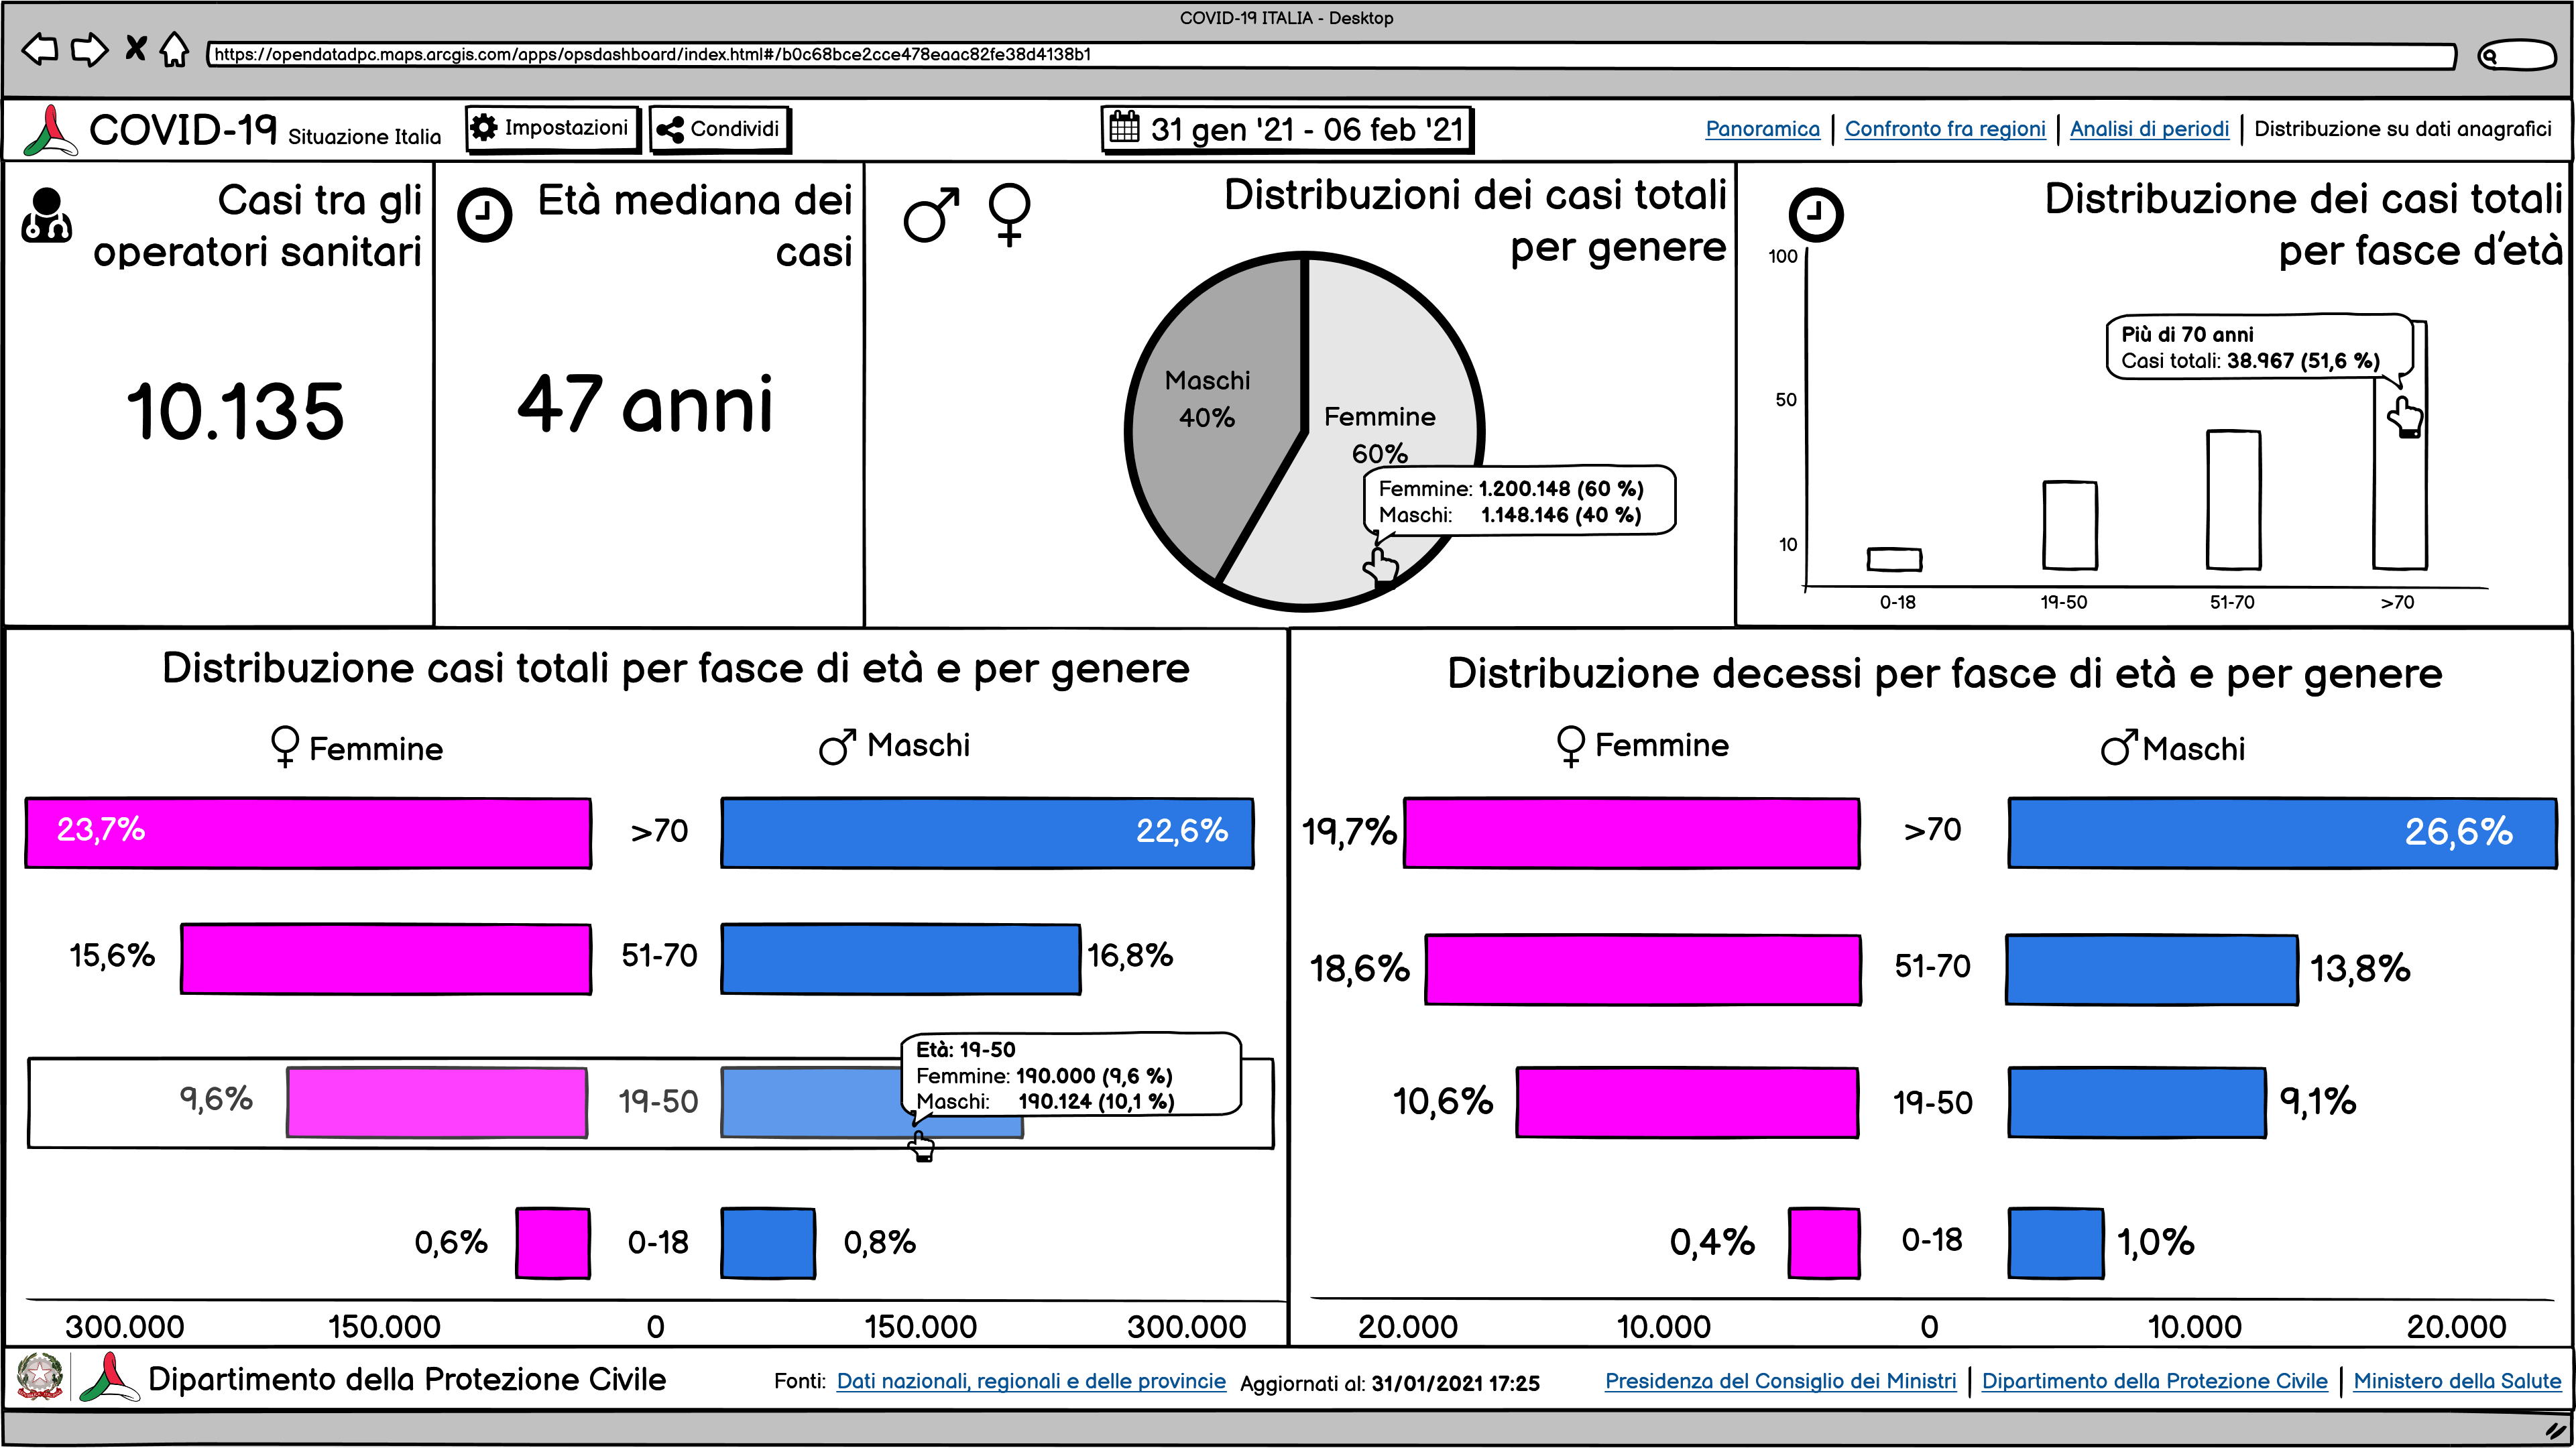
\includegraphics[trim = 0 459 0 53, clip, width=.7\textwidth]{screen-interfaccia/1 - Distribuzione su dati anagrafici}
        \caption{Parte alta della schermata "Distribuzione su dati anagrafici" dell'interfaccia riprogettata.}
    \end{figure}    

\end{frame}

\begin{frame}
    \frametitle{Distr. sui dati anagrafici - Distr. doppie}
    Nella parte bassa, sono mostrate distribuzioni doppie per età e genere.
    \begin{figure}
        \centering        
        \vspace{20pt}
        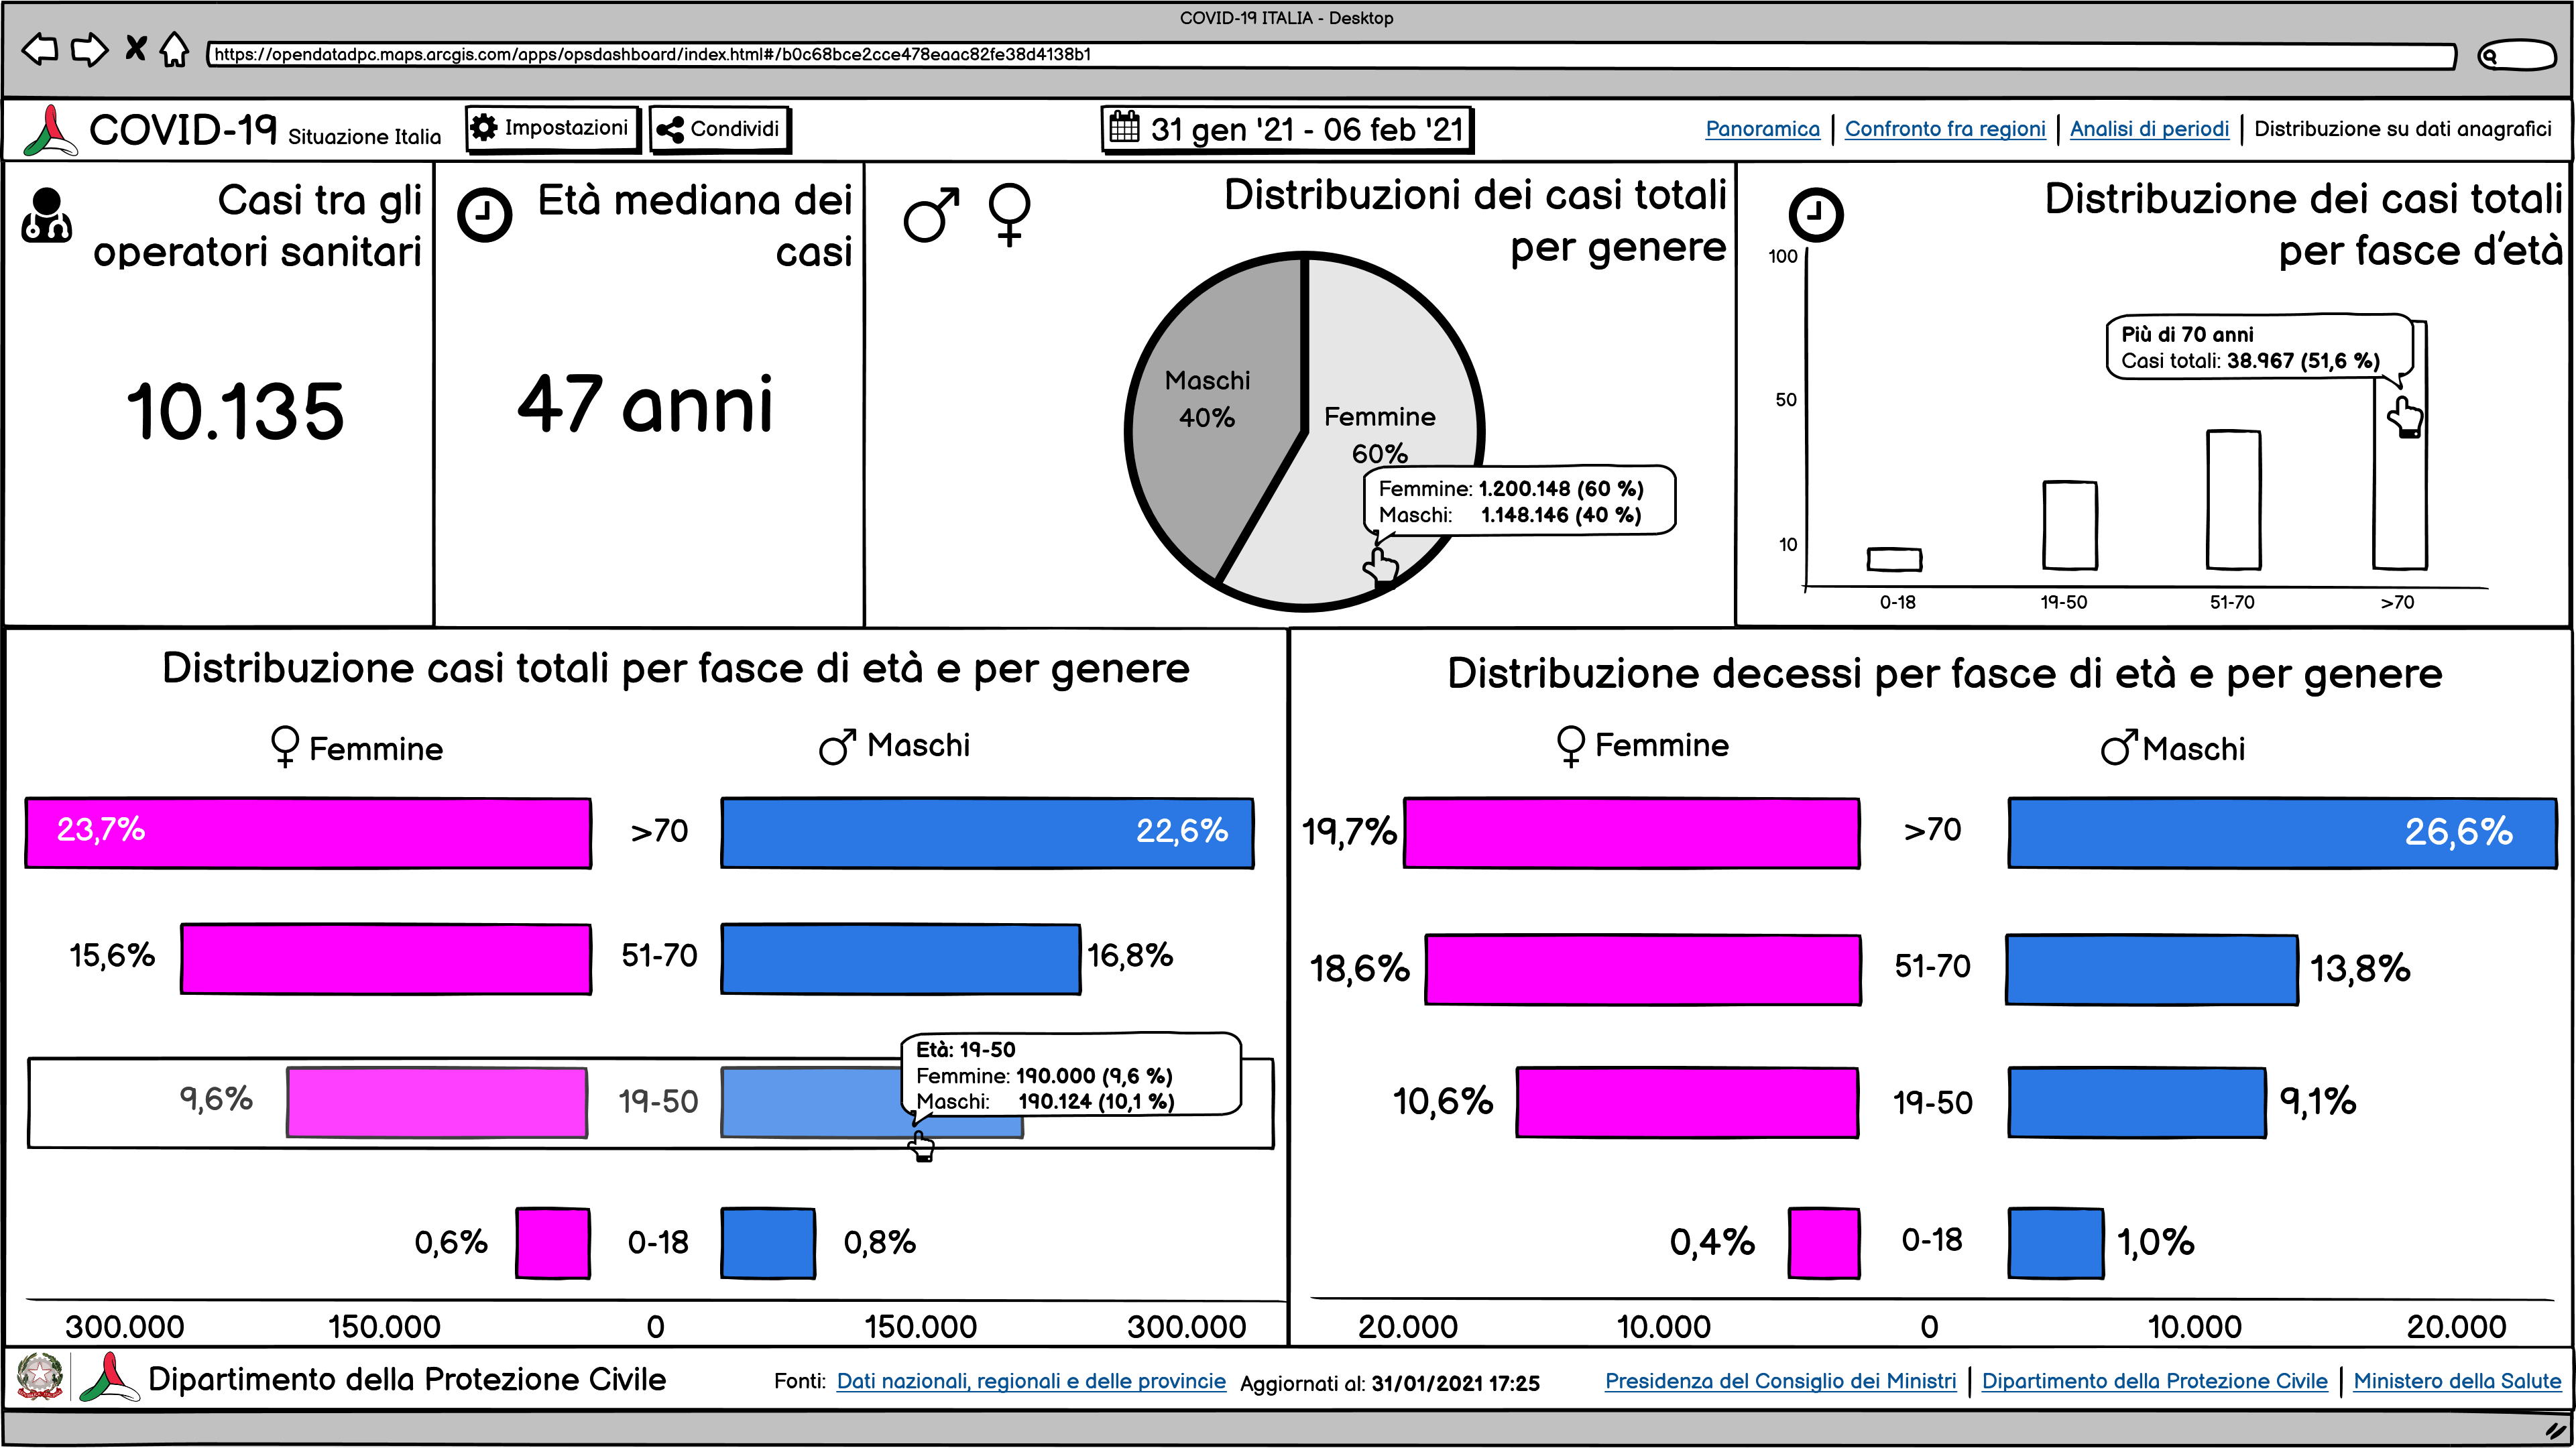
\includegraphics[trim = 0 20 0 350, clip, width=.7\textwidth]{screen-interfaccia/1 - Distribuzione su dati anagrafici}
        \caption{Parte bassa della schermata "Distribuzione su dati anagrafici" dell'interfaccia riprogettata.}
    \end{figure}    

\end{frame}
